\documentclass[
    table,
    12pt,
    oneside,
    a4paper,
    italian
]{book}

\PassOptionsToPackage{dvipsnames}{xcolor} % colori PDF/A

\usepackage{colorprofiles}
% PDF/A
% validate in https://www.pdf-online.com/osa/validate.aspx
\usepackage[a-1a,mathxmp]{pdfx}[2018/12/22]
\usepackage[T1]{fontenc}
\usepackage[utf8]{inputenc}
\usepackage[italian]{babel}
\usepackage{bookmark}
\usepackage{caption}
\usepackage{comment}
\usepackage{chngpage, calc} % centra il frontespizio
\usepackage{emptypage} % pagine vuote senza testatina e piede di pagina
\usepackage{epigraph} % per epigrafi
\usepackage{indentfirst} % rientra il primo paragrafo di ogni sezione
\usepackage{graphicx} % immagini
\usepackage[pdfa]{hyperref} % collegamenti ipertestuali
\usepackage{mparhack,relsize}  % finezze tipografiche
\usepackage{nameref} % visualizza nome dei riferimenti
\usepackage[font=small]{quoting} % citazioni
\usepackage{subfig} % sottofigure, sottotabelle
\usepackage[italian]{varioref} % riferimenti completi della pagina
\usepackage{longtable} % tabelle su più pagine
\usepackage[toc, acronym, automake]{glossaries}
\usepackage[backend=biber, style=verbose-ibid, hyperref, backref]{biblatex}
\usepackage{lmodern}
\usepackage[top=2.75cm, bottom=2.75cm, right=3cm, left=3.75cm]{geometry} % 1in+17pt+0.6cm
\usepackage{fancyhdr}
\usepackage{lipsum}
\usepackage{setspace}
\usepackage{titlesec}
\usepackage[cachedir=minted-caches]{minted} % https://it.overleaf.com/learn/latex/Code_Highlighting_with_minted
\usepackage{xcolor}
\usepackage{csquotes} % gestisce automaticamente i caratteri (")
\usepackage{etoolbox}
\usepackage[bottom]{footmisc}
\usepackage{zref-totpages}
\usepackage[italian]{babel}
\usepackage{tikz}
\usetikzlibrary{positioning, shapes, arrows.meta}
\usepackage{graphicx}
\usepackage{caption}
\usepackage{float}

% Load variables
\newcommand{\myUni}{Università degli Studi di Padova}
\newcommand{\myDepartment}{Dipartimento di Matematica ``Tullio Levi-Civita''}
\newcommand{\myFaculty}{Corso di Laurea in Informatica}
\newcommand{\myTitle}{Integrazione in gestionale ERP di un assistente virtuale basato su piattaforme di Intelligenza Artificiale}
\newcommand{\myDegree}{Tesi di Laurea}
\newcommand{\profTitle}{Prof.}
\newcommand{\myProf}{Vardanega Tullio}
\newcommand{\graduateTitle}{Laureando}
\newcommand{\myName}{Dal Bianco Riccardo}
\newcommand{\myStudentID}{2042385}
\newcommand{\myAA}{2024-2025}
\newcommand{\myLocation}{Padova}
\newcommand{\myTime}{Luglio 2025}
\input{references/glossary_acronyms}
\makeglossaries

% Define custom colors
\definecolor{hyperColor}{HTML}{0B3EE3}
\definecolor{tableGray}{HTML}{F5F5F7}
\definecolor{veryPeri}{HTML}{6667ab}

% Set line height
\linespread{1.5}

% Custom hyphenation rules
\hyphenation {
    data-base
    al-go-rithms
    soft-ware
}

% Images path
\graphicspath{{img/}}

% Force page color, as some editors set a grayish color as default
\pagecolor{white}

% Better spacing for footnotes
\setlength{\skip\footins}{5mm}
\setlength{\footnotesep}{5mm}

\setlength{\headheight}{14.5pt}
\addtolength{\topmargin}{-2.45pt}

% Add a subscript G to a glossary entry
\newcommand{\glox}{\textsubscript{\textbf{\textit{G}}}}

% Improvements the paragraph command
\titleformat{\paragraph}
{\normalfont\normalsize\bfseries}{\theparagraph}{1em}{}
\titlespacing*{\paragraph}
{0pt}{3.25ex plus 1ex minus .2ex}{1.5ex plus .2ex}

% Define use case environment
\newcounter{usecasecounter} % define a counter
\setcounter{usecasecounter}{0} % set the counter to some initial value
% Parameters
% #1: ID
% #2: Nome
\newenvironment{usecase}[2]{
    \renewcommand{\theusecasecounter}{\usecasename #1}  % this is where the display of the counter is overwritten/modified
    \refstepcounter{usecasecounter} % increment counter
    \vspace{2em}
    \par \noindent % start new paragraph
    {\normalsize \textbf{\usecasename #1: #2}} % display the title before the content of the environment is displayed
    \vspace{.5em}
}{
    \medskip
}
\newcommand{\usecasename}{UC}
\newcommand{\usecaseactors}[1]{\textbf{\\Attori Principali:} #1}
\newcommand{\usecasepre}[1]{\textbf{\\Precondizioni:} #1}
\newcommand{\usecasedesc}[1]{\textbf{\\Descrizione:} #1}
\newcommand{\usecasepost}[1]{\textbf{\\Postcondizioni:} #1}
\newcommand{\usecasealt}[1]{\textbf{\\Scenario Alternativo:} #1}

% Define risks environment
\newcounter{riskcounter} % define a counter
\setcounter{riskcounter}{0} % set the counter to some initial value
% Parameters
% #1: Title
\newenvironment{risk}[1]{
    \refstepcounter{riskcounter} % increment counter
    \par \noindent % start new paragraph
    \textbf{\arabic{riskcounter}. #1} % display the title before the content of the environment is displayed
}{
    \par\medskip
}
\newcommand{\riskname}{Rischio}
\newcommand{\riskdescription}[1]{\textbf{\\Descrizione:} #1.}
\newcommand{\risksolution}[1]{\textbf{\\Soluzione:} #1.}

% Apply fancy styling to pages
\pagestyle{fancy}
\fancyhf{}
\fancyhead[L]{\leftmark} % Places Chapter N. Chatper title on the top left
\fancyfoot[C]{\thepage} % Page number in the center of the footer

% Adds a blank page while increasing the page number
\newcommand\blankpage{ 
\clearpage
    \begingroup
    \null
    \thispagestyle{empty}
    \hypersetup{pageanchor=false}
    \clearpage
\endgroup
}

% Adds a blank page while increasing the page number
\newcommand\blankpagewithnumber{ 
  \clearpage
  \thispagestyle{plain} % Use plain page style to keep the page number
  \null
  \clearpage
}

% Increase page numbering
\newcommand\increasepagenumbering{
    \addtocounter{page}{+1}
}

% Make glossaries and bibliography
\makeglossaries
% Redefine the format for the glossary entries to be italic
\renewcommand*{\glstextformat}[1]{\textit{#1}\glox}
%\newcommand{\mygls}[2]{\hyperlink{gls:#1}{\textit{#2}\textsubscript{\textbf{\textit{G}}}}}

%\glsaddall

\newcommand{\mygls}[1]{\hyperlink{gls:#1}{\textit{#1}\textsubscript{\textbf{\textit{G}}}}}




\bibliography{references/bibliography}
\defbibheading{bibliography} {
  \cleardoublepage
    \phantomsection
    \addcontentsline{toc}{chapter}{\bibname}
    \chapter*{\bibname\markboth{\bibname}{\bibname}}
}

% Code blocks handling w/ table of codes
\makeatletter
\ifdefined\NR@chapter
  \expandafter\@firstoftwo
\else
  \expandafter\@secondoftwo
\fi{\patchcmd\NR@chapter}{\patchcmd\@chapter}
  {\addtocontents{lot}{\protect\addvspace{10\p@}}}
  {\addtocontents{lot}{\protect\addvspace{10\p@}}%
   \addtocontents{lol}{\protect\addvspace{10\p@}}}
  {}{}
\makeatother

\renewcommand\listingscaption{Codice}
\renewcommand\listoflistingscaption{Elenco dei codici sorgenti}
\counterwithin*{listing}{chapter}
\renewcommand\thelisting{\thechapter.\arabic{listing}}

% Set up hyperlinks
\hypersetup{
    colorlinks=true,
    linktocpage=true,
    pdfstartpage=1,
    pdfstartview=,
    breaklinks=true,
    pdfpagemode=UseNone,
    pageanchor=true,
    pdfpagemode=UseOutlines,
    plainpages=false,
    bookmarksnumbered,
    bookmarksopen=true,
    bookmarksopenlevel=1,
    hypertexnames=true,
    pdfhighlight=/O,
    allcolors = hyperColor
}

% Set up captions
\captionsetup{
    tableposition=top,
    figureposition=bottom,
    font=small,
    format=hang,
    labelfont=bf
}

% When draft mode is on, the hyperlinks are removed. Useful when printing the document. To enable/disable, uncomment/comment the command
% \hypersetup{draft}

% prevents cleaning up the cache at the end of the run (needed to keep the unused caches, generated by other editions)
\makeatletter
\renewcommand*{\minted@cleancache}{}
\makeatother

% Break lines in code blocks whe using inputminted
\setminted{breaklines}


\date{}

\hypersetup{pdfstartview=}
\begin{document}
    \frontmatter
    \begin{titlepage}
    \begin{center}
        \begin{Large}
            \textbf{\myUni}\\
        \end{Large}

        \vspace{5pt}

        \begin{large}
            \textsc{\myDepartment}\\
        \end{large}

        \vspace{5pt}

        \begin{large}
            \textsc{\myFaculty}\\
        \end{large}

        \vspace{25pt}
        
        \begin{figure}[htbp]
            \centering
            
\includegraphics[alt={Emblema dell'Università degli Studi di Padova}, height=6cm]{img/logo_unipd.jpeg}
        \end{figure}

        
        \begin{Large}
            \textbf{\myTitle}\\
        \end{Large}

        \vspace{5pt}

        \begin{large}
            \textit{\myDegree}\\
        \end{large}

        \vspace{50pt}
        
        \begin{normalsize}
            \begin{flushleft}
                \textit{Relatore}\\
                \profTitle\ \myProf
            \end{flushleft}

            \vspace{-48pt}
            
            \begin{flushright}
                \textit{\graduateTitle}\\
                \myName\\
                Matricola \myStudentID
            \end{flushright}
        \end{normalsize}

        \vspace*{\fill}
        
        \line(1, 0){338} \\
        \begin{normalsize}
            \textsc{Anno Accademico \myAA}
        \end{normalsize}
    \end{center}
\end{titlepage}

    \increasepagenumbering % increase the page numbrering by 1, in order to cout the frontispiece
    \clearpage
\phantomsection
\thispagestyle{empty}
\hfill
\vfill

{\small\noindent\textcopyright\ \myName, \myTime. Tutti i diritti riservati. \myDegree: ``\textit{\myTitle}'', \myUni, \myDepartment, \myFaculty.}
    \cleardoublepage
\phantomsection
\pdfbookmark{Ringraziamenti}{Ringraziamenti}

\begin{flushright}{
    \slshape
    Cacio e Pepe \\}
\end{flushright}

\begingroup
\let\clearpage\relax
\let\cleardoublepage\relax
\let\cleardoublepage\relax

\chapter*{Ringraziamenti}

\noindent 
\vspace{0.35cm}

\noindent \textit{Innanzitutto, desidero esprimere la mia gratitudine al Professor Tullio Vardanega, relatore della mia tesi, per il sostegno, l'aiuto e la disponibilità dimostrati durante la stesura della relazione finale.}

\vspace{0.35cm}

\noindent \textit{Ringrazio Francesco Turra, amministratore di VisioneImpresa, e tutti i ragazzi che vi lavorano per l'accoglienza e il supporto che mi hanno offerto durante l'intero periodo di stage.}

\vspace{0.35cm}

\noindent \textit{Con infinito affetto, desidero ringraziare i miei genitori per tutto l'appoggio e il sostegno che mi hanno sempre fornito durante questo percorso. Mi hanno permesso di inseguire i miei sogni, nonostante tutti i sacrifici che hanno dovuto fare.}

\vspace{0.35cm}

\noindent\textit{Voglio ringraziare Sara: non era con me all'inizio, ma da quando è arrivata tutto è cambiato. Ha sempre creduto in me più di quanto riuscissi a farlo io.}

\vspace{0.35cm}

\noindent \textit{Infine, un grazie va ai PADLUGHI, Baggio (Peter), Riki e Cri perché siete proprio così come siete e spero che questo non cambi mai.}

\vspace{0.75cm}

\noindent{\myLocation, \myTime}
\hfill \textit{\myName}

\endgroup

    \cleardoublepage
\phantomsection
\pdfbookmark{Compendio}{Compendio}
\begingroup
\let\clearpage\relax
\let\cleardoublepage\relax
\chapter*{Sommario}

Il presente documento descrive il lavoro svolto dal laureando Dal Bianco Riccardo durante il periodo di \textit{stage} svolto presso l'azienda VisioneImpresa.
La relazione di fine \textit{stage} si divide in quattro capitoli:
\begin{enumerate}
		\item Presentazione dell'azienda, informazioni generali su VisioneImpresa, i suoi prodotti, tecnologie utilizzate e propensione all'innovazione.
		\item  Contestualizzazione del progetto di \textit{stage} all'interno della strategia aziendale, perché è stato proposto e aspettative aziendali e personali.
		\item Descrizione delle attività svolte durante il periodo di \textit{stage}: l'analisi, la progettazione, parte dello sviluppo, la validazione e i risultati conseguiti.
		\item Raggiungimento degli obiettivi prefissati, valutazione e retrospettiva del periodo di \textit{stage} e del percorso universitario.
\end{enumerate}

\textbf{Convenzioni tipografiche} \\
All'interno del documento vengono utilizzate le seguenti convenzioni tipografiche:
\begin{itemize}
	\item \textit{Corsivo} indica i termini in lingua non italiana.
	\item \textbf{Grassetto} utilizzato negli elenchi puntati per enfatizzare la parola chiave e utilizzato nei titoli per enfatizzare le porzioni di testo.
	\item \texttt{Monospaziato} utilizzato per indicare nomi di funzioni, \textit{database}, tabelle, \textit{file} e classi.
	\item Parole del Glossario, rappresentate in corsivo, in blu e da una G a pedice (ad esempio \mygls{ERP}).
\end{itemize}

\endgroup
\vfill

    \cleardoublepage
\pdfbookmark{\contentsname}{tableofcontents}
\setcounter{secnumdepth}{5}
\setcounter{tocdepth}{5}     

\tableofcontents
\clearpage

\begingroup
    \let\clearpage\relax
    \let\cleardoublepage\relax
    \let\cleardoublepage\relax

    % Figures list
    \phantomsection
    \pdfbookmark{\listfigurename}{lof}
    \listoffigures
    \vspace*{8ex}

    % Tables list
    \phantomsection
    \pdfbookmark{\listtablename}{lot}
    \listoftables
\endgroup

\begingroup
    % Code list
    %\phantomsection
    %\pdfbookmark{\listoflistingscaption}{lol}
    %\listoflistings
\endgroup

\cleardoublepage

    

    
    \blankpage % example of a blank page that also increases the page couter by 1

    \mainmatter
    \chapter{Contesto aziendale}
\label{chap:Contesto-aziendale}


\section{VisioneImpresa}

VisioneImpresa è un'azienda con oltre quarant'anni di esperienza nel settore dell'\textit{Information Technology}. La sua attività è focalizzata sullo sviluppo di soluzioni \textit{software} per l'automazione e l'organizzazione di processi aziendali. In particolare, offre una gamma di strumenti \mygls{ERP}, sistemi integrati che permettono di gestire e coordinare in modo centralizzato le attività operative, dalla contabilità alla logistica, ottimizzando la gestione delle informazioni in un ambiente condiviso.

La sede si trova a Pernumia (PD), all'interno di un casolare ristrutturato nel cuore del territorio delle Terme Euganee ed ospita un \textit{team} di circa venti persone. VisioneImpresa opera prevalentemente nel Nord Est, ma con contatti che si estendono su tutto il territorio nazionale.

Nel 2016 è entrata a far parte del gruppo OfficeGroup, un \textit{network} di aziende orientate alla progettazione di \textit{software} gestionali avanzati. L'ingresso in questa rete ha favorito la crescita soprattutto grazie allo scambio di conoscenze e competenze con altre aziende andando a rafforzare la posizione di mercato.

Il 5 ottobre 2023, VisioneImpresa diventa una società \textit{benefit}, come viene indicato sul sito aziendale \footcite{site:vsh-sb}, non è stata una scelta imposta ma è arrivata attraverso un lungo e consapevole percorso.
Questa forma giuridica rappresenta le società che affiancano agli obiettivi di profitto anche attività che portano al beneficio comune. 

\begin{figure}[H]
    \centering
    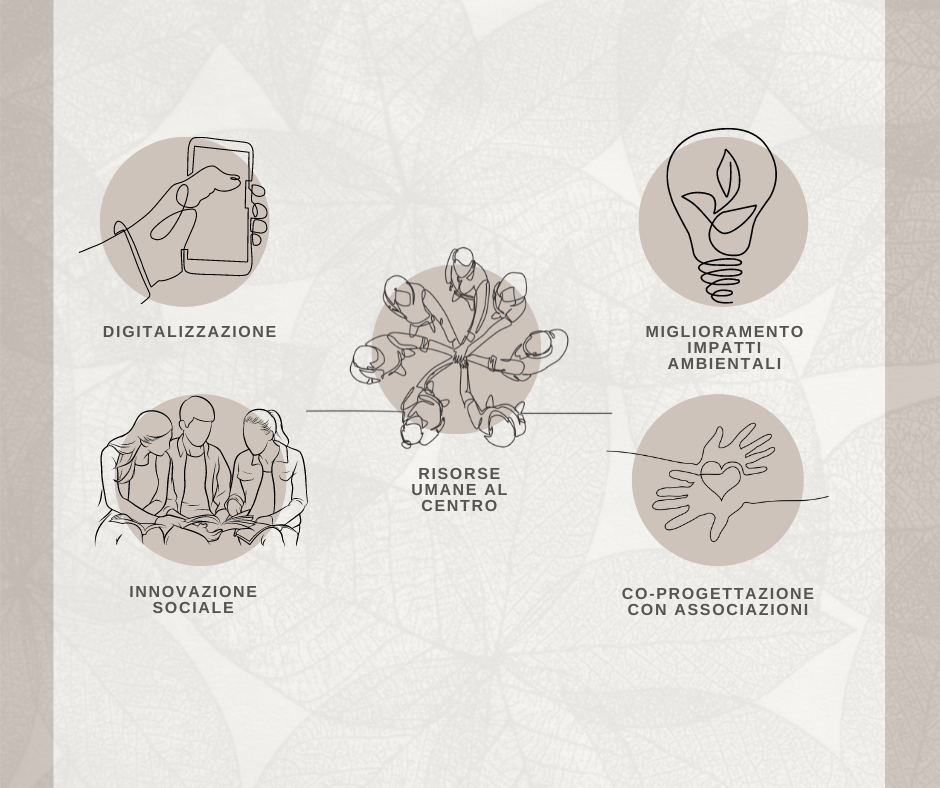
\includegraphics[alt={obiettivi società \textit{benefit}}, width=.5\columnwidth]{img/Sbenefit.png}
    \caption[Obiettivi di VisioneImpresa in quanto società \textit{benefit}.]{obiettivi di VisioneImpresa in quanto società \textit{benefit}. \\ \textit{fonte: \url{https://www.vsh.it/azienda/societa-benefit/}}}
    \label{fig:Benefit}
\end{figure} 

In qualità di società \textit{benefit} VisioneImpresa adotta una visione imprenditoriale responsabile, sostenibile e trasparente; assumendo impegni verso la società e l'ambiente.

Come dimostra la figura \ref{fig:Benefit} si impegna a perseguire i seguenti obiettivi:
\begin{itemize}
    \item La promozione della digitalizzazione al fine anche dell'utilizzo di minore quantità di materiali supportando la transizione ecologica.
    \item Il miglioramento delle condizioni lavorative, mettendo al centro il benessere delle risorse umane, riponendo particolare attenzione a tematiche come la parità di genere, la formazione continua e la conciliazione tra attività lavorativa e vita privata.
    \item La promozione di progetti orientati all'innovazione e al benessere sociale favorendo la collaborazione con enti del territorio tra cui scuole e università.
    \item Partecipazione attiva in progetti locali, favorendo la collaborazione con enti del territorio per generare valore alla comunità.
    \item Mantenere un'alta attenzione all'impatto ambientale, impegnandosi nell'utilizzo di risorse energetiche pulite e riducendo l'impatto attraverso pratiche legate al consumo di risorse e alla gestione dei rifiuti.
\end{itemize}

% ----------------------------------------------------------------

\section{Clienti e servizi}

% -----------------------------------------------------------

VisioneImpresa si rivolge principalmente a realtà di piccole e medie dimensioni situate nel Nord Est, ma opera anche in regioni del Centro Italia e in Sardegna. La principale offerta si fonda su soluzioni gestionali configurabili in base alle esigenze specifiche del cliente, affiancate da servizi di supporto tecnico e di consulenza. 
Il prodotto principale dell'azienda è VisionENTERPRISE, un sistema \mygls{ERP} modulare progettato per adattarsi a praticamente tutti i contesti aziendali.

\begin{figure}[H]
    \centering
    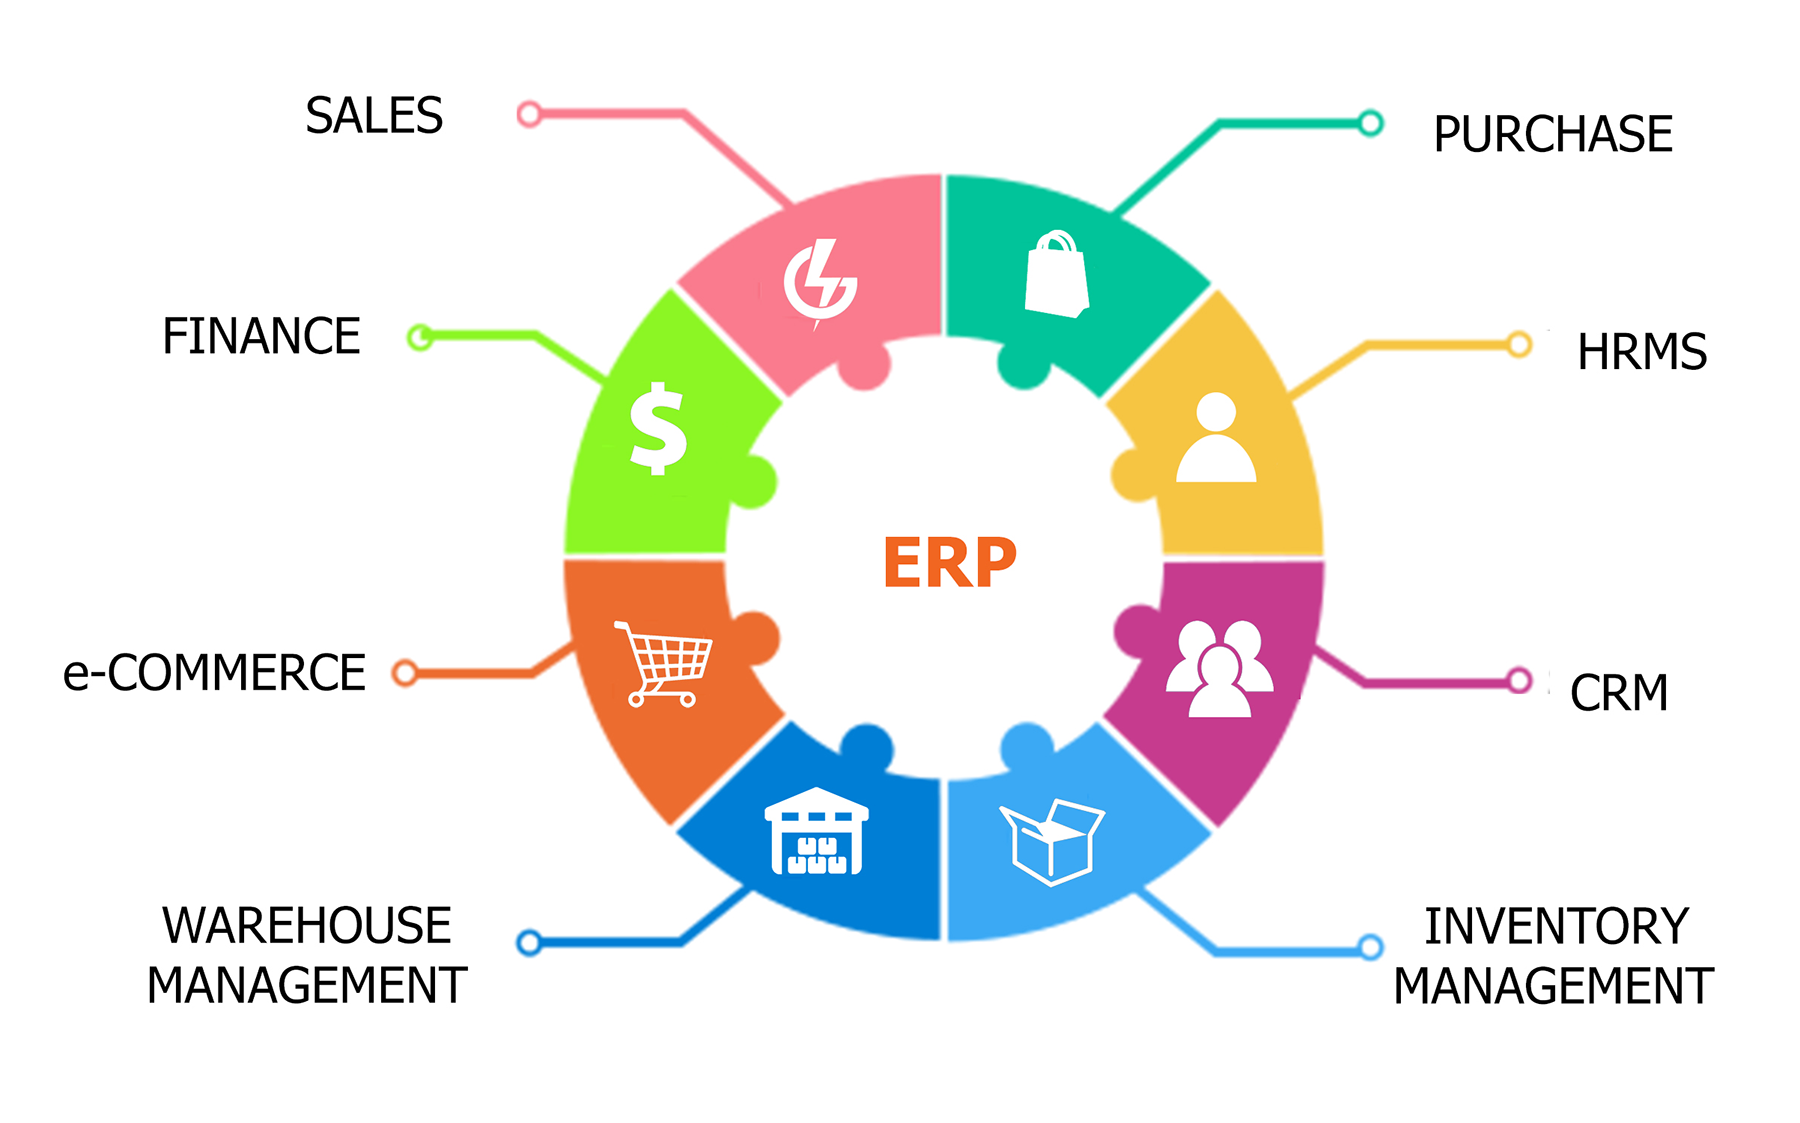
\includegraphics[alt={Enterprise Resource Planning}, width=1\columnwidth]{img/software-erp.png}
    \caption[Enterprise Resource Planning.]{Enterprise Resource Planning. \\ \textit{fonte: \url{https://www.softplaceweb.com/erp-open-source/}}}
    \label{fig:ERP}
\end{figure} 

Si tratta di un sistema flessibile, che costituisce una base alla quale vengono affiancate anche soluzioni verticali pensate per settori specifici. Questi prodotti verticali si basano sulla stessa infrastruttura \textit{software}, ma dispongono di funzionalità specifiche che hanno l'obiettivo di soddisfare esigenze particolari di determinate filiere produttive. \\


\textbf{Soluzioni verticali della linea Vision}\\
Le soluzioni verticali offerte da VisioneImpresa includono:
\begin{itemize}
\item \textbf{VisionENERGY:} Gestionale pensato per aziende del settore petrolifero, include diverse funzionalità, in aggiunta a quelle tipiche di un \mygls{ERP}, mirate a soddisfare bisogni di questo settore come la gestione della vendita del carburante, la manutenzione degli impianti, la fatturazione con defiscalizzazione e la manutenzione degli impianti.


\item \textbf{VisionBLUE:} Gestionale pensato per la filiera ittica, fornisce strumenti per attività legate alla vendita all'ingrosso dei prodotti ittici, come la gestione della tracciabilità dei prodotti, funzioni per l'inventario e organizzazione in contesti di alta intensità.


\item \textbf{VisionASSISTANCE:} Gestionale dedicato alle aziende che forniscono assistenza su prodotti, consente di gestire richieste di intervento, stipulazione di contratti di assistenza, organizzazione dei tecnici sul territorio e assegnazione di interventi.

\item \textbf{VisionFRESH:} Prodotto ideato per risolvere le esigenze del settore ortofrutticolo, contiene funzionalità che si integrano con le bilance elettriche, gestione dei lotti, imballaggi e prodotti e movimentazione della merce. 

\item \textbf{VisionANTINCENDI:} Gestionale che va a risolvere le richieste specifiche del settore della sicurezza e manutenzione di sistemi antincendio, offre funzionalità per la gestione degli interventi, gestione dei buoni di manutenzione e gestione dei contratti.


\item \textbf{VisionTRASPORTI:} Gestionale orientato alle aziende di logistica e trasporti, contiene funzionalità specifiche per facilitare la gestione dei listini, delle anagrafiche oppure funzionalità per la pianificazione dei tragitti.

\item \textbf{VisionELETTRO:} Gestionale dedicato alle officine elettromeccaniche, contiene funzionalità dedicate come la gestione delle matricole, gestione delle attività e navigazione per consultare lo storico degli interventi.

\end{itemize}

\textbf{Servizi di supporto e personalizzazione}\\
Oltre alla linea di prodotti principale VisioneImpresa offre diversi servizi accessori, tra questi ci sono un servizio di formazione rivolto al personale aziendale per istruirli all'utilizzo ottimale del \textit{software}, un servizio di assistenza tecnica in caso di problemi, un servizio di aggiornamento e manutenzione.
L'azienda inoltre offre la possibilità di effettuare personalizzazioni \textit{ad-hoc} su richiesta, queste personalizzazioni sono vere e proprie modifiche al \textit{software} di base per andare a risolvere esigenze mirate dei clienti, integrandole direttamente a livello del codice per mantenere stabile il sistema originario e fornire il massimo livello di prestazioni.


\textbf{La linea MoviDat}\\
In parallelo al gestionale principale, VisioneImpresa ha sviluppato una \textit{suite} di applicazioni mobili, che si chiama MoviDat, creata per facilitare le attività in mobilità. Le applicazioni si integrano in modo nativo con i gestionali Vision e permettono di interagire con esso quando l'utilizzo del \textit{computer} risulterebbe scomodo o impossibile. 
La linea MoviDat è composta da applicazioni per dispositivi mobili e compatibili con sistemi IOS o Android. L'obiettivo di questi prodotti è migliorare la fruibilità del gestionale semplificando azioni specifiche utilizzando in modo diretto uno \textit{smartphone} o un \textit{tablet}.
Fanno parte della linea MoviDat le seguenti applicazioni: \textit{MoviDoc, Han-dy, MoviSell, MoviRep, MoviAlert, MoviCheck, MoviExpenses, MoviCheckin,
MoviOrder} e \textit{MoviShop}.


\section{Processi aziendali}

\subsection{Metodologie}
Per quanto riguarda l'organizzazione delle attività l'azienda adotta metodologie Agile per la gestione dei progetti \textit{software}. Questa tipologia di organizzazione si basa su cicli di lavoro brevi e ben definiti chiamati \textit{sprint} la cui struttura può essere visualizzata nella figura \ref{fig:Agile}. 
Questi \textit{sprint} consentono al \textit{team} di adattarsi in maniera rapida ai cambiamenti concentrandosi nel migliorare il prodotto in maniera progressiva favorendo la comunicazione continua e riducendo il rischio di disallineamenti interni.

\begin{figure}[H]
    \centering
    
\includegraphics[alt={Agile}, width=.5\columnwidth]{thesis/files/img/metodo_agile.png}
    \caption[Struttura generale di un processo Agile.]{Struttura generale di un processo Agile. \\ \textit{fonte: \url{https://www.josoft.it/sviluppo-software-personalizzato/}}}
    \label{fig:Agile}
\end{figure} 

In particolare VisioneImpresa applica il \textit{framework} Scrum, uno dei modelli più utilizzati nell'ambito Agile. Scrum prevede la suddivisione di un periodo lungo in \textit{sprint} dalla durata fissa, di solito di 1-2 settimane, ognuno dei quali ha i propri obiettivi specifici e mira ad apportare un incremento al progetto.
L'immagine seguente mostra la struttura tipica del ciclo Scrum \ref{fig:Scrum}.

\begin{figure}[H]
    \centering
    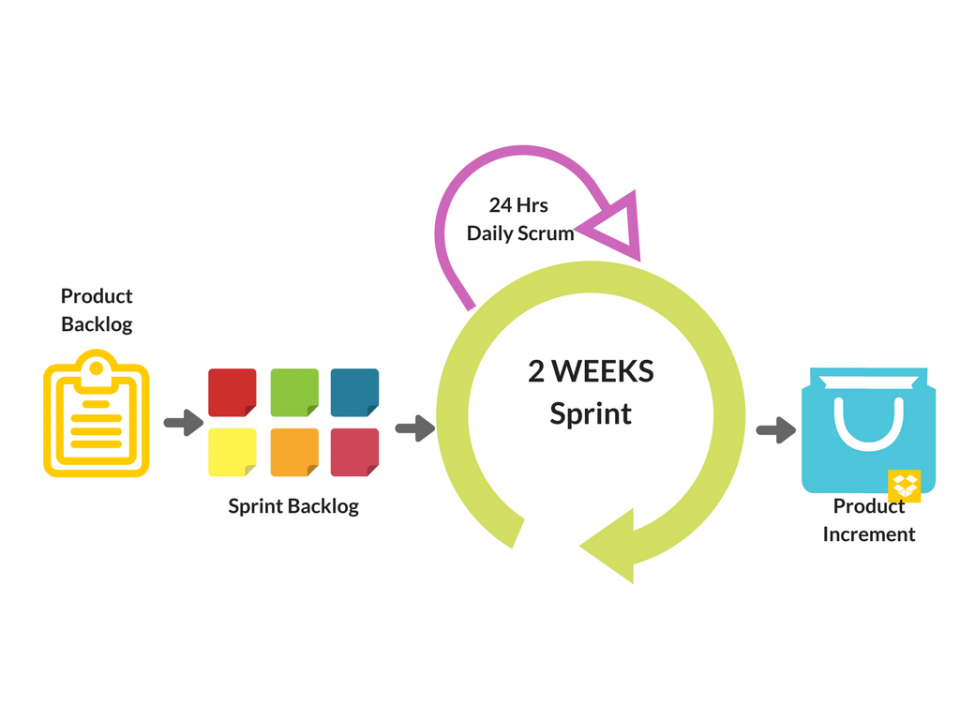
\includegraphics[alt={Scrum}, width=1\columnwidth]{thesis/files/img/Differenza-tra-Sprint-e-Sprint-Backlog-nella-metodologia-Agile-960x720.png}
    \caption[Ciclo di lavoro generale secondo Scrum.]{Ciclo di lavoro generale secondo Scrum. \\ \textit{fonte:\url{https://vitolavecchia.altervista.org/differenza-tra-sprint-e-sprint-backlog-nella-metodologia-agile/}}}
    \label{fig:Scrum}
\end{figure} 

Il \textit{framework} sopra presentato definisce un insieme di ruoli, ed eventi, così come descritti nella \textit{Scrum Guide} \footcite{misc:Guida-Scrum}. \\
Tuttavia, nel contesto di VisioneImpresa l'approccio Scrum non viene seguito in modo scolastico ma viene adottato con coerenza in alcuni casi specifici. 
In particolare, ho avuto modo di osservare direttamente la metodologia con il quale questo \textit{framework} viene applicato al progetto pluriennale di riscrittura del sistema gestionale VisionENTERPRISE, di cui fornirò più informazioni nella sotto-sezione \ref{Propensione-all'-innovazione}.
L'approccio adottato in questo contesto mantiene i principi fondamentali di questo metodo di lavoro, quali collaborazione, \textit{feedback}, trasparenza, ma presenta alcune personalizzazioni legate alle esigenze aziendali. \\
L'applicazione concreta del metodo si può riassumere nei seguenti punti:

\begin{itemize}
    \item \textbf{\textit{Sprint meeting} settimanali:}
    ogni mercoledì viene organizzata una riunione tecnica a cui partecipano gli sviluppatori coinvolti nel progetto. Questo incontro svolge sia la funzione di \textit{sprint planning} dove si discute degli obiettivi e delle funzionalità da implementare nel prossimo periodo, ma anche la funzione di \textit{sprint review} dove viene visualizzato il lavoro svolto nel periodo passato valutandone gli obiettivi conseguiti. Questa riunione viene fatta con l'obiettivo di discutere delle problematiche incontrate e fissare gli obiettivi per il prossimo periodo.
    \item \textbf{\textit{Daily meeting}:}
    ogni giorno gli sviluppatori partecipano a una breve \textit{call}, posizionata durante la mattinata, durante la quale tutti espongono cosa hanno fatto nel giorno precedente e quello in cui si concentrerà nella giornata corrente. Questo incontro viene svolto nel \textit{software} 3CX, il centralino telefonico usato per le comunicazioni interne, ed è fondamentale per mantenere tutto il \textit{team} allineato.
    \item \textbf{Flessibilità del lavoro:} 
    un'altra caratteristica osservata è che gli sviluppatori non hanno un carico di lavoro uniforme ma vengono destinate alla realizzazione del progetto, per motivi aziendali, risorse limitate, infatti lavorano a questo progetto solo alcuni giorni della settimana. Questa scelta è motivata dall'impossibilità di interrompere le attività e i processi legati al vecchio \textit{software}. Per questo motivo il \textit{team} deve gestire il lavoro con grande flessibilità per evitare blocchi o disallineamenti che rappresentano un rischio per lo sviluppo.
    \item  \textbf{Riunione mensile aziendale:}
    oltre alle attività settimanali, VisioneImpresa organizza un \textit{meeting} mensile a cui partecipano tutti i membri dell'azienda. Durante questo incontro vengono presentati gli avanzamenti conseguiti durante il mese, si fa il punto della situazione riguardante lo stato dei progetti in corso e si presenta quello che verrà fatto nel prossimo mese. Oltre a un compito di allineamento, questa riunione serve anche per favorire il dialogo tra tutti i componenti dell'azienda, i dipendenti infatti sono invitati a proporre soluzioni a eventuali problemi che sono stati individuati, avanzare idee e offrire punti di riflessione utili allo sviluppo dei progetti, sia attuali che futuri. Questa fase può essere vista come una sessione di \textit{brainstorming} aziendale dove viene stimolato un confronto sui temi trattati.
\end{itemize}
Per concludere, l'adozione del modello Scrum da parte di VisioneImpresa non segue una struttura rigida, ma si configura secondo le esigenze progettuali. Nonostante tutto questo processo, visto da un occhio esterno, risulta coerente con i principi fondamentali e si dimostra efficace nell'organizzare e coordinare un progetto di grandi dimensioni come questo.


\subsection{Tecnologie e strumenti utilizzati}
Nel contesto di competenza nel quale opera, VisioneImpresa utilizza un ampia \textit{gamma} di tecnologie a supporto delle attività. Questi strumenti possono essere divisi in base al contesto di utilizzo ovvero: strumenti operativi, strumenti per la comunicazione e la produttività, strumenti per lo sviluppo \textit{software}, strumenti per la gestione del codice e dei progetti.
Essendo così grande il numero di tecnologie impiegate e non essendo entrato in contatto con tutti gli ambiti dell'azienda, le tecnologie descritte in seguito sono solo quelle che ho avuto modo di osservare o quelle con cui ho avuto il modo di interagire durante il periodo di \textit{stage}.

\textbf{Strumenti operativi}
\begin{itemize}
  \item Portatili aziendali: ad ogni dipendente viene fornito un portatile personale, con sistema operativo Windows 10 o 11, oppure macOS. 
  \item Dispositivi mobili: per i dipendenti che si occupano di sviluppo di applicazioni \textit{mobile} vengono dati in dotazione \textit{smartphone} e/o \textit{tablet} con sistemi Android o IOS, utilizzati principalmente per funzioni di \textit{testing} delle applicazioni.
\end{itemize}

\textbf{Strumenti per la comunicazione e la produttività}
\begin{itemize}
  \item Microsoft Office 365: \textit{suite} di strumenti Microsoft per la produttività.
  \item Outlook: client integrato, facente parte della \textit{suite} Office, utilizzato per la posta elettronica e per la comunicazione interna e esterna.
  \item 3CX: centralino telefonico \mygls{PBX}, una tecnologia che consente creare una rete di comunicazioni interna, utilizzato per le chiamate vocali, messaggistica istantanea e riunioni online. 
\end{itemize}

\textbf{Strumenti per lo sviluppo \textit{software}}
\begin{itemize}
  \item Visual Studio: Un \mygls{IDE} un ambiente di sviluppo che contiene strumenti per scrivere e testare codice progettato da Microsoft. Molto utilizzato nei progetti che coinvolgono il \textit{framework} .NET , data una larga \textit{gamma} di strumenti offerti.
  \item Visual Studio Code: \textit{editor} di codice sorgente \textit{open-source}, sviluppato da Microsoft, viene contraddistinto per la sua leggerezza, velocità e personalizzazione.
  \item SQL Server Management Studio (SSMS): Questo strumento è dedicato alla gestione dei \textit{database} relazionali basati su SSMS, ha un interfaccia molto esplicativa e viene utilizzato per la gestione in tempo reale dei dati.
  \item Swagger: Piattaforma per la progettazione e la documentazione di \mygls{API} \mygls{REST}, ovvero interfacce che permettono la comunicazione tra sistemi \textit{web}, permette di visualizzare in maniera chiara le chiamate, e offre strumenti per testare le richieste e le risposte.
\end{itemize}
\textbf{\textit{Framework} e linguaggi}
\begin{itemize}
  \item .NET: Un \textit{framework} di sviluppo \textit{software} creato da Microsoft che consente lo sviluppo di vari applicazioni sia a livello \textit{desktop} sia a livello \textit{mobile} e \textit{web}. 
  \item FoxPro: Linguaggio di programmazione e sistema per la gestione del \textit{database}, attualmente considerato \textit{\mygls{legacy}} a causa della dismissione ufficiale del supporto da parte di Microsoft nel 2015. Viene utilizzato per la manutenzione in attesa della completa migrazione verso tecnologie più moderne.
\end{itemize}

\textbf{Gestione del codice e dei progetti}
\begin{itemize}
  \item Bitbucket: Strumento utilizzato per il versionamento del codice e facilitare la collaborazione tra membri del \textit{team}. Offre funzionalità di controllo delle modifiche e revisione del codice. 
  \item Jira: Strumento sviluppato da Atlassian per la gestione dei progetti e la divisione delle \textit{task}. Supporta le metodologie Agile consentendo la gestione del lavoro in \textit{sprint}.
  \item Excel: Nonostante sia uno strumento che non offre le stesse potenzialità di altri come Jira, viene utilizzato per la pianificazione elementare delle attività.
\end{itemize}

\textbf{Integrazione delle tecnologie nei processi aziendali} \\
Durante il periodo di \textit{stage} ho potuto osservare come gli strumenti e le tecnologie vengono integrate all'interno del flusso di lavoro. Nello schema seguente \ref{fig:strumenti-integrazione} viene rappresentato in maniera semplificata l'integrazione dei principali strumenti all'interno dei processi aziendali, come osservato durante la mia esperienza.

\begin{figure}[H]
\centering
\begin{tikzpicture}[
    box/.style={
        draw, rectangle,
        text width=3.4cm, align=center,
        minimum height=1.2cm, font=\small
    },
    arrow/.style={thick, ->, >=Stealth},
    node distance=1.2cm and 1.4cm
]

% Riga superiore
\node[box] (doc) {Documentazione\\\textbf{Word, Excel}};
\node[box, right=of doc] (comm) {Comunicazione\\\textbf{3CX, \\Outlook, Teams}};
\node[box, right=of comm] (task) {Gestione Attività\\\textbf{Jira, Excel}};

% Nodo centrale
\node[box, below=1.4cm of comm, text width=9cm, minimum height=2.4cm] (dev) {
\textbf{Sviluppo \textit{software}}\\
.NET, C\# $\rightarrow$ Visual Studio / VS Code\\
SQL Server $\rightarrow$ SQL Server Management Studio\\
API Testing: Swagger
};

% Frecce principali verso sviluppo
\draw[arrow] (doc.south) -- ([xshift=-2.5cm]dev.north);
\draw[arrow] (comm.south) -- (dev.north);
\draw[arrow] (task.south) -- ([xshift=2.5cm]dev.north);

% Nuove frecce laterali da "Comunicazione"
\draw[arrow, bend left=20] (comm.west) to (doc.east);
\draw[arrow, bend right=20] (comm.east) to (task.west);

% Nodo inferiore
\node[box, below=1.2cm of dev] (versioning) {Controllo Versione\\\textbf{Bitbucket (Git)}};
\draw[arrow] (dev.south) -- (versioning.north);

\end{tikzpicture}
\caption[Schema di integrazione degli strumenti nei processi aziendali]{
Schema semplificato dell'integrazione degli strumenti principali nei processi aziendali.
}
\label{fig:strumenti-integrazione}
\end{figure}

Di seguito è presentato nel dettaglio come ciascun processo aziendale viene affiancato e supportato dalle tecnologie citate.

\begin{itemize}

    \item \textbf{Documentazione} \\
    La scrittura della documentazione avviene principalmente attraverso Microsoft Word, con il quale vengono redatti i documenti più significativi, come le analisi dei requisiti e i casi d'uso, solitamente questa attività viene svolta dal responsabile di progetto e in seguito i documenti vengono condivisi con il \textit{team} di sviluppo. Nel mio periodo di \textit{stage}, ho preso visione di diversi documenti e ne ho scritti alcuni. Inoltre, vengono prodotti anche i documenti a supporto delle riunioni, che svolgono il ruolo di verbali, riportando i temi trattati. L'utilizzo di Excel si limita ad alcuni casi specifici.
    
    \item \textbf{Comunicazione} \\
    Lo strumento principale per quanto riguarda la comunicazione interna è 3CX, utilizzato per chiamate, messaggi istantanei e riunioni. È lo strumento preferito per la collaborazione rapida tra i membri dell'azienda. Io non ho avuto un account per l'accesso a 3CX e ho comunicato con Microsoft Outlook, utilizzandolo per mandare e leggere mail e messaggi. In alcune occasioni come la riunione aziendale mensile viene utilizzato Microsoft Teams .


    \item \textbf{Gestione attività} \\
    Le attività inerenti ai progetti vengono tracciate utilizzando principalmente Jira, ma talvolta a livello di supporto viene impiegato anche Microsoft Excel per via della sua semplicità. Durante il mio \textit{stage} i miei compiti erano assegnati via email o tramite riunioni in presenza, non ho utilizzato quindi in prima persona strumentazione per la gestione delle attività.

    \item \textbf{Sviluppo \textit{software}} \\
    Per quanto riguarda lo sviluppo \textit{software} le tecnologie e i linguaggi adottati variano in base al progetto di riferimento. Per la mia esperienza il \textit{framework} di riferimento è .NET, utilizzato con il linguaggio C\#, viene usato per lo sviluppo di applicazioni \textit{web} e \textit{desktop} in maniera performante. Gli ambienti di sviluppo variano sempre in base al progetto di riferimento ma principalmente vengono utilizzati Visual Studio o Visual Studio Code. Tutte le applicazioni sviluppate si interfacciano con \textit{database} relazionali gestiti tramite SQL Server Management Studio (SSMS), questo strumento viene utilizzato per la creazione, la manutenzione e l'interrogazione del \textit{database}.
    Per quanto riguarda le \mygls{API} \mygls{REST}, VisioneImpresa utilizza Swagger come strumento di testing e documentazione, favorendo la visualizzazione dei risultati e migliorando lo sviluppo.

    \item \textbf{Controllo versione} \\
    Per quanto riguarda invece la gestione del codice in azienda viene utilizzato Bitbucket. Anche se non mi sono interfacciato direttamente con i \textit{repository}, ho visualizzato alcuni flussi tipici del codice. Il codice di ogni progetto viene messo in \textit{repository} dedicati, i quali poi sono strutturati in \textit{branch} come \textit{main}, \textit{develop} e \textit{branch} specifici per implementare funzionalità.
    Questo strumento consente di mantenere il codice stabile e versionato, migliorando lo sviluppo in parallelo.
   
\end{itemize}

\section{Propensione all'innovazione}
\label{Propensione-all'-innovazione}
VisioneImpresa non dispone di un reparto dedicato alla ricerca e sviluppo, ciononostante l'innovazione e l'aggiornamento rappresentano un elemento fondamentale sulla quale si basa la filosofia aziendale. 
Essendo un'azienda che opera da oltre quarant'anni nel settore dell'\textit{Information Technology}, ha avviato un processo di transizione tecnologica di ampio raggio, tra le iniziative più significative c'è la progressiva migrazione dei sistemi \mygls{ERP} sviluppati in FoxPro verso ambienti più moderni e performanti. Questo processo per complessità e dimensione richiede una pianificazione pluriennale e il coinvolgimento graduale di un gran numero di risorse.
In parallelo a questa transizione, VisioneImpresa considera i progetti di \textit{stage} un'opportunità concreta per il progresso. Durante il mio tirocinio, ho avuto modo di contribuire attivamente allo sviluppo di progetti finalizzati alla modernizzazione. In particolare mi è stato comunicato che uno dei due progetti a cui ho avuto modo di lavorare è destinato a integrarsi con il nuovo gestionale attualmente in fase di sviluppo, pensato per sostituire l'attuale \mygls{ERP} con una soluzione più moderna e tecnologicamente avanzata.
Inoltre, l'azienda incoraggia gli stagisti a proporre nuove idee e soluzioni tecniche, introducendo anche nuove tecnologie in autonomia. Questa libertà consente di testare nuove soluzioni in un ambiente controllato, favorendone la possibile introduzione nei processi aziendali.

\newpage
    \chapter{Definizione del percorso di stage}
\label{chap:Definizione-del-percorso-di-stage}

\section{Il rapporto tra azienda e \textit{stage}}
Come già accennato nella sotto-sezione \ref{Propensione-all'-innovazione}, VisioneImpresa investe molte risorse nei progetti di \textit{stage}, ritenendo che questi siano uno strumento concreto ed efficace per promuovere l'innovazione e la sperimentazione.
Durante il mio periodo di tirocinio erano presenti, oltre a me, altri quattro \textit{stagisti}. Quasi tutti erano impegnati in progetti differenti e ritenuti rilevanti dall'azienda. Questo dato testimonia quanto VisioneImpresa ritenga importante questo tipo di rapporto con gli studenti e gli enti del territorio. In quanto società \textit{benefit} l'azienda persegue anche obiettivi sociali, tra i quali la collaborazione con scuole e università attraverso progetti orientati all'innovazione.
Gli \textit{stagisti} provengono principalmente da corsi di laurea triennali in informatica o ingegneria informatica, portando con loro le conoscenze accademiche acquisite negli anni. Lo \textit{stage} ha una durata di 300-320 ore un tempo che consente allo studente di contribuire in maniera concreta allo sviluppo di soluzioni aziendali, e allo stesso tempo conferisce un esperienza significativa dal punto di vista professionale.
I progetti presentati dall'azienda non hanno un obiettivo prettamente formativo, ma corrispondono a necessità reali dell'azienda, emerse tramite il confronto con clienti o con \textit{team} di sviluppo interni. I tirocinanti si trovano quindi immersi nel contesto aziendale con l'obiettivo di affrontare problematiche concrete, analizzare e riscrivere codice esistente e approfondire tecnologie, situazioni spesso nuove per uno studente.
Alla fine del periodo ciascun tirocinante presenta il lavoro svolto al \textit{team} di sviluppo più appropriato e al referente aziendale, questa fase è cruciale per rendere possibile la valutazione del lavoro svolto e spiegare il progetto da un punto di vista tecnico ponendo le basi per una possibile futura integrazione di esso nei prodotti aziendali.
Inoltre VisioneImpresa utilizza il periodo di \textit{stage} anche come momento per valutare il profilo dello studente, sia a livello tecnico che a livello personale. In diversi casi, il tirocinio si è trasformato in un'opportunità concreta di inserimento nel contesto lavorativo, rendendo possibile agli studenti di proseguire il percorso all'interno dell'azienda.



\section{Proposte progettuali dell'azienda}
Il primo contatto con VisioneImpresa è avvenuto grazie l'evento StageIT 2025, organizzato dall'università di Padova per mettere in contatto studenti alla ricerca di un tirocinio e aziende del territorio che propongono offerte di \textit{stage} in ambito informatico. 
Durante l'evento ho avuto modo di svolgere numerosi colloqui con aziende interessanti, che proponevano una vasta scelta di progetti distribuiti su molti ambiti applicativi.
Nonostante durante l'evento no abbia svolto un colloquio diretto con VisioneImpresa, sono stato contattato nei giorni seguenti tramite \textit{email}. In questo messaggio era presente un invito a leggere le proposte progettuali dell'azienda e nel caso ne fossi stato interessato la possibilità di effettuare un colloqui direttamente in sede per approfondire la conoscenza.
In seguito a questo primo contatto ho svolto un riunione dove mi è stato possibile conoscere il referente aziendale, approfondire le proposte progettuali e avere un primo approccio con l'ambiente di lavoro. Durante questa visita mi sono presentati numerosi progetti di \textit{stage}, tutti con obiettivi e ambiti di applicazione differenti, la tabella  \ref{tab:Proposte-progetto} contiene una visuale generale delle proposte di progetto dell'azienda.

\begin{longtable}{|p{4.2cm}|p{11cm}|}
\caption{Proposte di progetto presentate da VisioneImpresa.} \\
\hline
\textbf{Nome progetto} & \textbf{Breve descrizione} \\
\hline
\endfirsthead

\hline
\textbf{Nome progetto} & \textbf{Breve descrizione} \\
\hline
\endhead

VisionAI & Progetto mirato all'espansione di un assistente virtuale esistente in grado di rispondere in linguaggio naturale, interrogando il \textit{database} aziendale. Il tirocinante lavorerà al fine di ottimizzare le \mygls{API} già esistenti e crearne di nuove, inoltre lavorerà alla creazione di un \textit{agent} intelligente. \\
\hline
\textit{WebApp} attivazione istanze & Sviluppo di una \textit{webapp} interna all'azienda che ha l'obiettivo di automatizzare le configurazioni di nuove installazioni \textit{software}, generazione cartelle, \textit{database}, utenti, credenziali, PDF, e invio automatico di mail.\\
\hline
Catalogo multimediale moviSELL & Sviluppo di un modulo integrato per l'\textit{app} moviSELL. L'obiettivo è la creazione di un catalogo interattivo con immagini e video dove l'utente può svogliare il suddetto catalogo, selezionare i prodotti e inserirli nel carrello. \\
\hline
Versione lite moviREP & Creazione di una versione \textit{smartphone} dell'\textit{app} moviREP, che condivide i dati con la versione per tablet ma offre un'interfaccia più essenziale. \\
\hline
Siti \textit{web} a basso impatto ambientale & Ottimizzazione di siti WordPress e PrestaShop per andare a ridurre l'impatto ambientale, andando a diminuire i consumi energetici e migliorando le prestazioni. \\
\hline
moviEXPENSE con OCR & Aggiornamento dell'\textit{app} moviEXPENSE, facendo la migrazione a React Native e aggiungendo un sistema OCR per l'estrazione automatica di dati da scontrini. \\
\hline
moviSELL \textit{Web} & Progettazione e sviluppo dell'\textit{app} nativa per dispositivi \textit{mobile} moviSLL. L'obiettivo è andare a replicare le funzionalità principali della versione \textit{tablet}, connettendola con il \textit{database}. \\
\hline
\textit{Report Designer} moviSELL/moviREP & Sviluppo di un modulo per la creazione di \textit{report} personalizzati in PDF per le \textit{app} moviSELL e moviREP, utilizzando strumenti integrati nell'applicazione. \\
\hline
Gestione multilingua & Aggiungere la funzionalità di supporto multilingua delle descrizioni dei prodotti e delle tabelle correlate all'interno delle \textit{app} moviSELL e moviREP, adattando il testo in automatico alla lingua dell'utente. \\

\hline
\caption{Panoramica delle proposte progettuali.}
\label{tab:Proposte-progetto}
\end{longtable}


Questa offerta progettuale così ampia testimonia in quanti ambiti tecnologici differenti lavora VisioneImpresa e sottolinea il valore conferito ai progetti di \textit{stage}, tutti orientati a a fornire risposte a esigenze concrete dell'azienda.





\section{Valutazione e presentazione del progetto}

\subsection{Valutazione e scelta}
Ho scelto il progetto di \textit{stage} in seguito a una attenta valutazione delle proposte disponibili, l'azienda ha presentato un ampio ventaglio di proposte progettuali spaziando in molti contesti di sviluppo differenti.
Tra i progetti disponibili ho scelto, in accordo con il \textit{tutor} aziende, il progetto 1, VisionAI, incentrato sullo sviluppo di un sistema intelligente in grado di fornire risposte in linguaggio naturale a domande poste dagli utenti, interrogando in modo diretto il \textit{database} aziendale.
Ho deciso di intraprendere questo progetto principalmente per un forte interesse personale per il settore dell'intelligenza artificiale e della sua applicazione. In particolare, sono molto interessato nell'osservare da vicino come queste tecnologie trovino applicazioni in ambienti lavorativi, anche in realtà di medie-piccole dimensione. Mi interessa inoltre il comprendere quali sono i processi decisionali che portano all'adozione di suddette tecnologie in sistemi funzionanti, e di come le persone possono rapportarsi con essi.


\subsection{Presentazione del progetto}
\label{subs:Presentazione-progetto}

Il progetto selezionato nasce dal concetto base di introdurre soluzioni intelligenti all'interno dei propri prodotti \textit{software}, con l'obiettivo di mantenere le applicazioni e i servizi offerti competitivi all'interno di un settore in continua evoluzione. 
L'idea è quella di semplificare l'accesso alle informazioni, integrando tecnologie che permettono l'utilizzo del linguaggio naturale e inoltre automatizzare processi decisionali complessi.
Il lavoro è stato concepito come progetto unitario, articolato in due componenti distinte che però condividono le stesse finalità.
Il primo componente riguarda  VisionAI, un assistente virtuale, del quale alla base c'è già un prototipo funzionante, capace di interagire via chat con l'utente per fornire risposte a domande di base, interrogando il \textit{database} per ottenere le informazioni.
Lo scopo di questa sezione è sviluppare e perfezionare le \mygls{API} su cui VisionAI si basa, utilizzate per dialogare con il \textit{database}, aumentando così il raggio di azione dell'assistente e consentendogli di fornire risposte a domande più complesse.
La seconda parte riguarda lo sviluppo di un \textit{agent}, questo modulo basandosi sempre su dati presenti nel \textit{database}, ha come scopo quello di dare supporto alle aziende che operano nel campo dell'assistenza tecnica, organizzando in modo efficace l'ordine degli interventi in un determinato periodo, cercando di ottimizzare l'assegnazione dei tecnici agli interventi da svolgere.
In conclusione, sebbene il progetto è diviso in due sezioni distinte, mantiene una visione coerente e unitaria, orientata ad integrare nei prodotti aziendali strumenti "intelligenti".

\subsection{Vincoli generali del progetto}
Come in tutti i progetti nel mondo reale, anche il progetto di stage è sottoposto a vincoli esterni, imposti sia dal contesto aziendale sia dalla pianificazione temporale del tirocinio. Ovviamente questi vincoli hanno un influenza nelle scelte tecnologiche e organizzative prese nelle varie fasi di sviluppo.

\textbf{Vincoli temporali}
\begin{figure}[H]
    \centering
    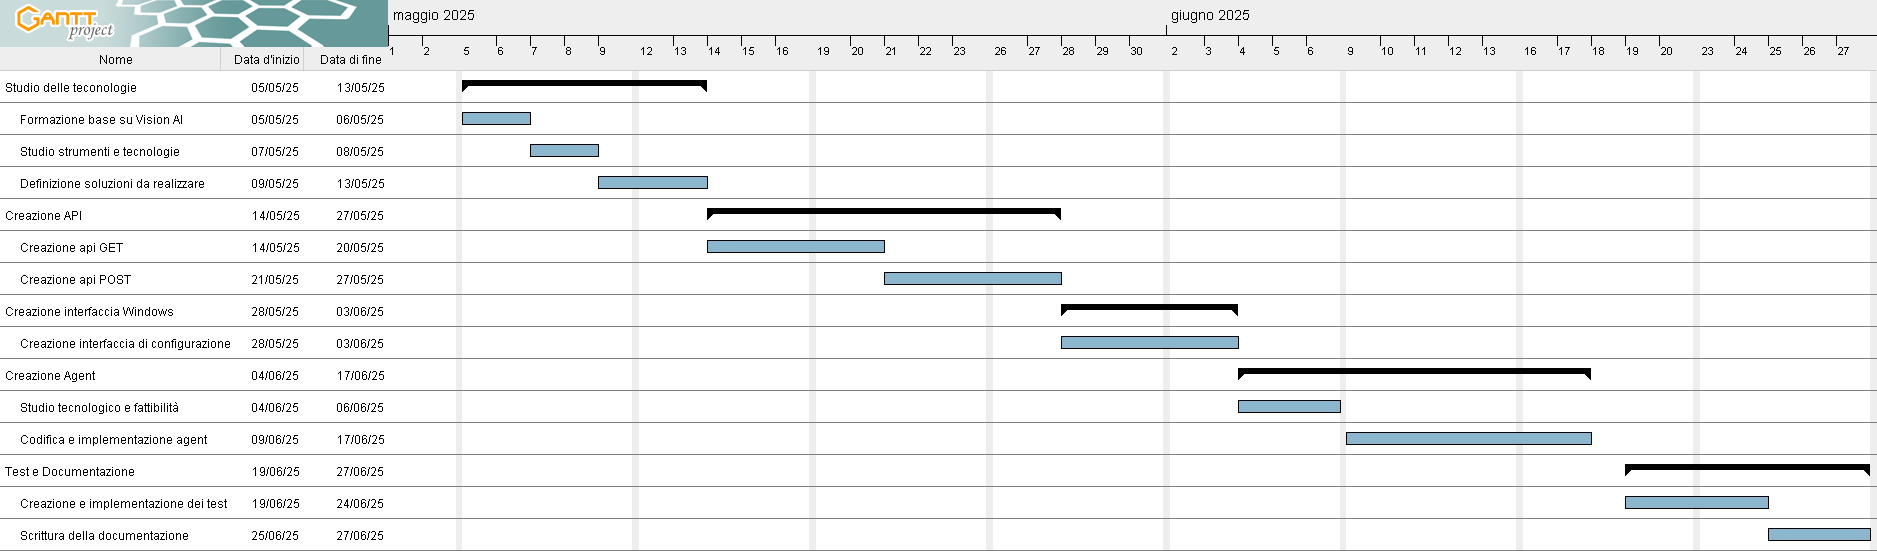
\includegraphics[width=\textwidth]{thesis/files/img/gaant.png}
    \caption{Pianificazione temporale dello \textit{stage}}
    \label{fig:pianificazione-stage}
\end{figure}

La struttura del lavoro all'interno del periodo di \textit{stage}, che è determinato da un monte ore limitato, è stata definita in collaborazione con il \textit{tutor} aziendale, suddividendo il tempo totale in sotto-periodi come illustrato nell'immagine \ref{fig:pianificazione-stage}. Questa divisione è avvenuta prima dell'inizio del tirocinio e presentata nel piano di lavoro.
Lo \textit{stage} è stato diviso in queste sezioni:
\begin{itemize}
    \item \textbf{Studio degli applicativi e del \textit{database}} (una settimana), l'obiettivo di questo periodo era l'apprendimento delle tecnologie e l'analisi del codice già presente, inoltre una prima formazione sulla struttura del \textit{database}.
    \item \textbf{Nuove \mygls{API}} (due settimane), in questo periodo è stata pianificata la creazione delle nuove \mygls{API} e perfezionare quelle già esistenti.
    \item \textbf{Interfaccia di configurazione} (una settimana), il periodo indicato allo sviluppo dell'interfaccia di connessione a VisionAI, creando un \textit{form} per la connessione al \textit{database} e alla \textit{chat}.
    \item \textbf{\textit{Agent}} (due settimane), l'obiettivo di questo periodo è la progettazione e lo sviluppo dell'\textit{agent} per la pianificazione automatica degli interventi.
    \item \textbf{\textit{Test} e documentazione} (una settimana e mezza), questo il periodo dedicato alla stesura della documentazione tecnica e allo svolgimento dei \textit{test}.
\end{itemize}

\textbf{Vincoli tecnologici generali}\\
L'azienda non ha imposto vincoli predefiniti a livello di tecnologie per la comunicazione e la documentazione, ma inserendosi in un contesto lavorativo già avviato comporta l'adozione di strumenti e metodologie già in uso.
% COMUNICAZIONE
\begin{figure}[H]
\centering
\begin{tikzpicture}[node distance=1cm and 2cm, every node/.style={font=\sffamily}, align=center]

  \node[draw, fill=white, minimum width=5.5cm, minimum height=3cm] (comunicazioni) at (0,0) {
    \textbf{Comunicazioni} \\[0.5em]
    \includegraphics[width=1cm]{thesis/files/img/Microsoft_Office_Outlook_(2018–present).svg.png} \\[-0.2em]
    Outlook \\[1em]
    \includegraphics[width=1cm]{thesis/files/img/Microsoft_Office_teams_(2018–present).svg.png} \\[-0.2em]
    Teams
  };

  \node[draw, fill=white, minimum width=5.5cm, minimum height=3cm, right=of comunicazioni] (doc) {
    \textbf{Documentazione} \\[0.5em]
    
\includegraphics[width=1cm]{thesis/files/img/word.png} \\[-0.2em]
    Word \\[1em]
    
\includegraphics[width=1cm]{thesis/files/img/2023_Obsidian_logo.svg.png} \\[-0.2em]
    Obsidian
  };
\end{tikzpicture}
\caption{Tecnologie utilizzate per la comunicazione e la documentazione.}
\label{fig:doc_com}
\end{figure}
La figura \ref{fig:doc_com} mostra le tecnologie utilizzate per le comunicazioni: 
\begin{itemize}
    \item Outlook: strumento di comunicazione utilizzato per lo scambio di posta elettronica con il referente aziendale o membri dei \textit{team} di sviluppo, per la gestione degli appuntamenti in calendario e per la pianificazione di incontri e riunioni.
    \item Microsoft Teams: strumento utilizzato in occasione della riunione mensile per rendere possibile la partecipazione di elementi non presenti direttamente in sede e per svolgere incontri di informazione organizzati dal \textit{tutor} aziendale con persone esterne.
\end{itemize}
 Gli strumenti per la documentazione sono i seguenti: 
 \begin{itemize}
     \item Microsoft Word: utilizzato principalmente per consultare e integrare la documentazione fornitaci dal \textit{tutor} aziendale e per integrare la seguente documentazione con i risultati dei \textit{test} svolti sul prodotto sviluppato.
     \item Obsidian: strumento utilizzato per redigere la documentazione tecnica in modo semplice e leggibile, utilizzato per organizzare appunti, annotazioni e idee durante il periodo di \textit{stage} tramite \textit{markdown}.
 \end{itemize}

 
\section{Vincoli tecnologici e obiettivi aziendali}
Il progetto come ho descritto nella sotto-sezione \ref{subs:Presentazione-progetto} è stato diviso in due componenti differenti, ognuno dei quali ha presentato vincoli tecnologici e obiettivi aziendali distinti.

\subsection{Assistente VisionAI}
L'azienda, come già detto, non impone vincoli tecnologici fissi, lasciando piena libertà nella decisione di linguaggi, \textit{framework} e ambienti di sviluppo.
Le scelte a livello di tecnologie da utilizzare quindi sono prese in maniera autonoma dallo stagista principalmente in base a efficacia e familiarità.
Nel caso specifico del progetto VisionAI, tuttavia, esisteva già una base di codice preesistente, sviluppata in C\#, e gli obiettivi concordati prevedevano espressamente l'utilizzo di questo linguaggio. In aggiunta durante lo sviluppo del prototipo iniziale erano già state prese anche altre scelte, è quindi stato opportuno mantenere lo \textit{stack} tecnologico già in uso per coerenza, visualizzabile nelle figure \ref{img:sviluppo} e \ref{fig:TecAI}

\textbf{Ambienti di sviluppo}
% SVILUPPO 
\begin{figure}[H]
\centering
\begin{tikzpicture}[node distance=2cm and 1.5cm, every node/.style={font=\sffamily}, align=center]

  % Blocco Sviluppo
  \node[draw, fill=white, minimum width=5cm, minimum height=3.8cm] (sviluppo) {
    \textbf{Ambienti di sviluppo} \\[0.5em]
    
\includegraphics[width=1cm]{thesis/files/img/vs.png} \\[-0.2em]
    Visual Studio \\[1em]
    
\includegraphics[width=1cm]{thesis/files/img/vscode.png} \\[-0.2em]
    Visual Studio Code \\[1em]
    
\includegraphics[width=1cm]{thesis/files/img/ssms.png} \\[-0.2em]
    SSMS
  };

\end{tikzpicture}
\caption{Ambienti di sviluppo per il modulo VisionAI.}
\label{img:sviluppo}
\end{figure}

\begin{itemize}
    \item Visual Studio: strumento utilizzato per la scrittura e il mantenimento del codice delle \mygls{API} tramite il supporto nativo al \textit{framework} .NET. scelto per i numerosi strumenti che fornisce a supporto dello sviluppo come strumenti di \textit{debug} e la gestione dei pacchetti.
    \item Visual Studio Code: utilizzato anche questo per lo sviluppo delle \mygls{API}, scelto principalmente per la familiarità con l'ambiente, per rendere più efficiente la scrittura del codice in determinati momenti.
    \item SQL Server Management Studio (SSMS): utilizzato per eseguire interrogazioni al \textit{database} relazione, supporta la scrittura di più \textit{query} in contemporanea e utilizzato per svolgere operazioni nel \textit{database} a supporto dello sviluppo.
\end{itemize}

\textbf{\textit{Framework} e \textit{software}}
\begin{figure}[H]
\centering
\begin{tikzpicture}[node distance=2cm and 2cm, every node/.style={font=\sffamily}, align=center]

  \node[draw, fill=white, minimum width=5.5cm, minimum height=4cm] (testing) at (0,0) {
    \textbf{\textit{Testing}} \\[0.5em]
    
\includegraphics[width=1cm]{thesis/files/img/swagger.png} \\[-0.2em]
    Swagger \\[1em]
    
\includegraphics[width=1cm]{thesis/files/img/postman.png} \\[-0.2em]
    Postman \\ [1em]
    
\includegraphics[width=1cm]{thesis/files/img/images.jpeg} \\[-0.2em]
    Ngrok 
  };

  \node[draw, fill=white, minimum width=5.5cm, minimum height=4cm, left=of testing] (API) {
    \textbf{Sviluppo \textit{API} e \textit{form}} \\[0.5em]
    
\includegraphics[width=1cm]{thesis/files/img/aspcore.png} \\[-0.2em]
    ASP.NET Core \\[1em]
    
\includegraphics[width=1cm]{thesis/files/img/entity_image.png} \\[-0.2em]
    Entity Framework \\[1em]
    
\includegraphics[width=1cm]{thesis/files/img/odata.png} \\[-0.2em]
    OData
  };

\end{tikzpicture}
\caption{Tecnologie utilizzate per il modulo VisionAI.}
\label{fig:TecAI}
\end{figure}
\begin{itemize}
    \item ASP.NET Core: \textit{framework} utilizzato per la scrittura delle \mygls{API} \mygls{REST}ful, permesso di sviluppare \mygls{endpoint}(url a cui un client può inviare richieste per eseguire operazioni sui dati) e mantenere alte le prestazioni
    \item Entity Framework Core: strumento \mygls{ORM}, tecnica che consente di interagire con \textit{database} in linguaggio di programmazione anzi che utilizzare \textit{query}, utilizzato per l'accesso ai dati.
    \item OData: Utilizzato per integrare funzionalità all'interno della \mygls{API} direttamente via URL, permettendo all'intelligenza artificiale di formulare \textit{query} con filtri direttamente all'interno dell'URL della chiamata
\end{itemize}

In merito alle tecnologie a supporto della fase di \textit{testing} delle \mygls{API} sono state:
\begin{itemize}
    \item Swagger: utilizzato per la generazione automatica della documentazione delle \mygls{API}, tramite la sua interfaccia inoltre è possibile esplorare le chiamate ed effettuare \textit{test} facilitando il \textit{debug}.
    \item Postman: tecnologia utilizzata per effettuare \textit{test} mirati, impiegato principalmente per \textit{testare} la funzionalità delle \mygls{API} POST.
    \item Ngrok: utilizzato per esporre in modo temporaneo il \textit{backend} e le \mygls{API} alla rete esterna, questo strumento ha permesso di \textit{testare} le chiamate all'interno della \textit{chat} senza dover pubblicare il servizio su un \textit{server} remoto.
\end{itemize}


\textbf{Obiettivi aziendali} \\
La tabella \ref{tab:obiettivi-aziendali} contiene gli obiettivi concordati con il \textit{tutor} aziendale previsti per la sezione corrente.
Gli obiettivi sono categorizzati in obbligatori, lettera O, desiderabili, lettera D, e facoltativi, lettera F.
\begin{table}[H]
\centering
\begin{tabular}{|c|p{11cm}|}
\hline
\textbf{Codice} & \textbf{Descrizione} \\
\hline
O01 & Sviluppo interfacce Visual Studio con librerie DevExpress \\
\hline
O02 & Sviluppo delle \mygls{API} di \textit{back-end} in linguaggio C\# \\
\hline
D01 & Creazione in autonomia della documentazione e del piano di \textit{test}  \\
\hline
\end{tabular}
\caption{Tabella obiettivi aziendali sezione VisionAI}
\label{tab:obiettivi-aziendali}
\end{table}


\subsection{Modulo di pianificazione interventi }
La sezione del progetto incentrata allo sviluppo dell'\textit{agent} per la pianificazione automatica degli interventi nel contesto di VisionAssistance è stato iniziato da zero, quindi ha concesso una libertà assoluta dal punto di vista tecnologico, la figura \ref{img:sviluppoa} mostra le scelte relative agli ambienti di sviluppo mentre la figura \ref{fig:Ag} mostra le scelte relative ai linguaggi e strumenti \textit{software} prese per questo modulo.

\textbf{Ambienti di sviluppo}
% SVILUPPO 
\begin{figure}[H]
\centering
\begin{tikzpicture}[node distance=2cm and 1.5cm, every node/.style={font=\sffamily}, align=center]

  % Blocco Sviluppo
  \node[draw, fill=white, minimum width=5cm, minimum height=3.8cm] (sviluppo) {
    \textbf{Ambienti di sviluppo} \\[0.5em]
    
\includegraphics[width=1cm]{thesis/files/img/vscode.png} \\[-0.2em]
    VS Code \\[1em]
    
\includegraphics[width=1cm]{thesis/files/img/ssms.png} \\[-0.2em]
    SSMS
  };

\end{tikzpicture}
\caption{Ambienti di sviluppo  per il modulo assegnazione interventi.}
\label{img:sviluppoa}
\end{figure}

\begin{itemize}
    \item Visual Studio Code: ambiente scelto per la scrittura del codice python, utilizzato per la familiarità con l'ambiente di sviluppo e la disponibilità di estensioni utili.
    \item SQL Server Management Studio (SSMS): impiegato per eseguire interrogazioni e operazioni sul \textit{database} aziendale, utile per la visualizzazione dei dati e verificare l'integrità dei dati utilizzati.

\end{itemize}

\textbf{Linguaggi e strumenti \textit{software}}

%\textit{agent}
\begin{figure}[H]
\centering
\begin{tikzpicture}[node distance=1cm and 2cm, every node/.style={font=\sffamily}, align=center]

  \node[draw, fill=white, minimum width=6cm, minimum height=3.5cm] (agent) at (0,0) {

    \textbf{Tecnologie \textit{software}} \\[0.5em]
    
\includegraphics[width=1cm]{thesis/files/img/python.png} \\[-0.2em]
    Python \\[1em]
    
\includegraphics[width=1cm]{thesis/files/img/sqlA.png} \\[-0.2em]
    SQLAlchemy \\[1em]
    
\includegraphics[width=1cm]{thesis/files/img/orLogo.png} \\[-0.2em]
    OR-Tools
  };

\end{tikzpicture}
\caption{Tecnologie utilizzate per il modulo di pianificazione interventi.}
\label{fig:Ag}
\end{figure}
\begin{itemize}
    \item Python: Linguaggio di programmazione principale utilizzato per lo sviluppo di questo progetto, scelto per la sintassi semplice, la familiarità e per la compatibilità con OR-Tools.
    \item SQLAlchemy: libreria \mygls{ORM} utilizzata per gestire l'accesso ai dati. Infatti, permette di scrivere \textit{query} in linguaggio SQL direttamente all'interno del codice per facilitare l'accesso ai dati.
    \item Google OR-Tools: \textit{solver} per la programmazione vincolata, è stato utilizzato per risolvere il problema dell'assegnazione ottimale degli interventi.
\end{itemize}

\textbf{Obiettivi aziendali}\\
La tabella \ref{tab:obiettivi-aziendali-interventi} contiene gli obiettivi concordati con il \textit{tutor} aziendale previsti per la sezione del progetto di stage in questione.
Il codice identificativo è il medesimo della sezione precedente.
\begin{table}[H]
\centering
\begin{tabular}{|c|p{11cm}|}
\hline
\textbf{Codice} & \textbf{Descrizione} \\
F01 &  Creazione di un \textit{agent} per la pianificazione degli interventi in VisionAssistance \\
\hline
\end{tabular}
\caption{Tabella obiettivi aziendali per sezione pianificazione interventi}
\label{tab:obiettivi-aziendali-interventi}
\end{table}







\section{Obiettivi personali}
La tabella \ref{tab:obiettivi-personali} mostra invece gli obiettivi personali stipulati prima dell'inizio dello \textit{stage}, la notazione degli obiettivi è la stessa delle tabelle precedenti.

\begin{table}[H]
\centering
\begin{tabular}{|c|p{11cm}|}
\hline
\textbf{Codice} & \textbf{Descrizione} \\
\hline
O01 & Imparare nuove tecnologie e \textit{framework} legati all'ambiente .NET e al linguaggio C\# \\
\hline
O02 & Collaborare attivamente con il \textit{team}, mantenendo una comunicazione efficace e continua \\
\hline
O03 & Svolgere le attività nel rispetto delle scadenze concordate. \\
\hline
D01 & Ampliare il mio bagaglio tecnico e di \textit{soft-skill} in un contesto strutturato \\
\hline
\end{tabular}
\caption{Obiettivi personali dello \textit{stage}.}
\label{tab:obiettivi-personali}
\end{table}




\newpage
    \chapter{Il progetto di stage}
\label{chap:I-progetti-di-stage}

\section {Pianificazione delle attività}
\label{sec:pianificazione-attività}
Come ho già anticipato nella sotto-sezione \ref{subs:Presentazione-progetto} abbiamo suddiviso il progetto di \textit{stage} in due sezioni separate, entrambe rivolte a migliorare le soluzioni aziendali fornendo soluzioni "intelligenti".
La prima fase del periodo ha riguardato l'estensione delle funzionalità dell'assistente virtuale interno al gestionale chiamato VisionAI mentre la seconda ha riguardato lo sviluppo di un sistema di assegnazione automatica con l'obiettivo di essere integrato all'interno di VisionAssistance.
La pianificazione delle attività non ha previsto l'utilizzo di \textit{software} specifici, abbiamo gestito il lavoro in maniera flessibile ponendo alla base la comunicazione con il \textit{tutor} aziendale, che ha avuto un ruolo importante sia per quanto riguarda l'organizzazione delle attività sia nel supporto formativo iniziale.
Lo \textit{stage} è stato svolto in coppia con un altro studente, con il quale ho condiviso lo spazio di lavoro e tutte le attività. Abbiamo collaborato costantemente avendo lavorato in maniera combinata a quasi tutte le porzioni del progetto, affrontando in maniera condivisa le problematiche e contribuendo entrambi alla buona riuscita del progetto.
L'unica distinzione ha riguardato la fase di sviluppo del modulo di assegnazione automatica, in cui abbiamo seguito lo sviluppo di parti diverse ma complementari, io mi sono occupato della \textit{pipeline} di raccolta e strutturazione dei dati, mentre il mio collega si è occupato dell'algoritmo di di assegnazione. Nonostante questa divisione abbiamo mantenuto una comunicazione costante che ha permesso l'integrazione tra le due componenti.
L'approccio per le attività può essere definito incrementale, con cicli della durata breve. Ogni inizio settimana veniva svolto un breve incontro con il \textit{tutor} aziendale, questi momenti seppur brevi erano molto utili per avere un \textit{feedback} sul lavoro svolto e ricevere linee guida per procedere al passo successivo.
Oltre agli incontri di persona, il \textit{tutor} forniva le attività anche tramite documentazione tecnica, contenti nuove funzionalità da implementare e note di contesto come \textit{query} di esempio inserite per rendere più facile la comprensione della struttura del \textit{database} e le relazioni tra le tabelle.
Ognuna delle due fasi è stata preceduta da un periodo di studio, necessario per familiarizzare con le tecnologie da utilizzare, comprendere i sistemi esistenti e l'infrastruttura \textit{software} aziendali. Per entrambi i casi questo periodo di studio è durato circa una settimana è stato fondamentale per poter procedere in maniera organizzata allo sviluppo vero e proprio. Durante queste fasi di molto importante è stata la creazione di appunti che sono stati utili in fase di sviluppo.



\section{Sviluppo di API REST per VisionAI}
In questa sezione descrivo la sezione di progetto finalizzata allo sviluppo delle \mygls{API} \mygls{REST} e l'ampliamento delle funzionalità dell'assistente interno chiamato VisionAI. Il lavoro si è concentrato su piccole migliorie delle \mygls{API} già presenti e l'integrazione di nuovi \mygls{endpoint}, rendendo il sistema capace di accedere a nuovi dati del \textit{database} aziendale.


\subsection{Contesto applicativo e funzionamento di VisionAI}
Al fine di comprendere appieno le scelte progettuali e le modalità di sviluppo è importante analizzare l'architettura preesistente e il funzionamento di VisionAI, così da dare contesto al lavoro svolto. L'infrastruttura \textit{software} si basa sull'integrazione tra un motore \mygls{LLM}, un modello di inteligenza artificiale avanzato che può comprendere e generare linguaggio naturale, gestito tramite un interfaccia sviluppata da DevLab e un \textit{backend} strutturato a microservizi \mygls{REST}.

\textbf{Architettura generale} \\
VisionAI è un assistente intelligente integrato in modo diretto all'interno del gestionale aziendale, ideato per rispondere a domande in linguaggio naturale e restituire informazioni prelevate da uno o più \textit{database} interni.
L'utente interagisce tramite una \textit{chat} e il motore sottostante si occupa:
\begin{itemize}
    \item analizzare e interpretare il significato della domanda,
    \item visualizzare le \mygls{API} a disposizione e selezionare quella più adatta,
    \item costruire la chiamata \mygls{HTTP} (protocollo di comunicazione per trasferimento dati sul web) con i parametri corretti per l'\mygls{API} in questione,
    \item trasformare la risposta ottenuta in testo comprensibile all'utente.
\end{itemize}

\textbf{Componenti del sistema}
\begin{enumerate}
    \item Motore realizzato da DevLab\\
    Il punto centrale del sistema è un motore \mygls{LLM} chiamato "mentiscrm". Questo strumento permette di configurare in modo dettagliato il comportamento dell'assistente con la possibilità di creare il \textit{prompt} principale che viene inviato in ogni iterazione fornendo il contesto necessario, definire le \mygls{API} \mygls{REST} che l'assistente può utilizzare, sarà poi il motore che gestisce la richiesta \mygls{HTTP}. Altra funzione importante è la possibilità di dare contesto tramite una descrizione alle singole \mygls{API} per permettere all'\mygls{LLM} di chiamare quella giusta e nel modo corretto.
    \item \textit{Frontend} realizzato da DevLab \\
    Interfaccia dell'assistente, si presenta come una classica \textit{chat} \mygls{LLM} 
    \item \textit{Backend} VisionAI \\
    Il \textit{backend} contenete le \mygls{API}, espone una serie di \mygls{endpoint} \mygls{REST}ful e contiene il codice sorgente scritto in C\# delle \mygls{API}
    \item Interazione con \mygls{LLM} \\
    Il motore realizzato da DevLab funziona da interfaccia tra la \textit{chat} dove scrive l'utente e il modello di \mygls{LLM} in questo caso GPT-4-mini.
\end{enumerate}

\textbf{Panoramica del flusso operativo}

\begin{figure}[H]
    \centering
    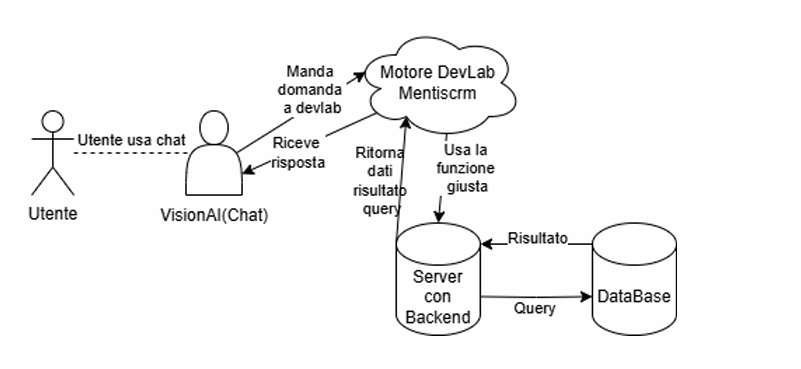
\includegraphics[width=\textwidth]{thesis/files/img/FlussoDatiVisionAI.PNG}
    \caption{Flusso operativo di VisionAI.}
    \label{fig:Architettura-generale}
\end{figure}

L'immagine \ref{fig:Architettura-generale} rappresenta il flusso di funzionamento di VisionAI, inizia con l'inserimento di una domanda in linguaggio naturale da parte dell'utente in \textit{chat}. Il motore di DevLab elabora la richiesta e utilizzando il modello GPT trova l'\mygls{API} più adatta per la richiesta,  successivamente costruisce in modo dinamico l'URL della chiamata. Il \textit{backend} elabora la richiesta, accede al \textit{database} e restituisce i dati in formato JSON. Per concludere GPT interpreta il risultato e crea una risposta in linguaggio naturale.


\subsection{Analisi dei requisiti}
L'analisi rappresenta uno dei momenti più importanti nell'ingegneria del \textit{software}, questa attività costituisce il momento in cui le idee e i bisogni vengono trasformate in specifiche operative che guideranno in seguito la fase di progettazione, sviluppo e validazione. 
L'analisi dei requisiti in particolare ha come scopo quello di identificare le funzionalità che il sistema deve offrire per rispondere alle necessità individuate dall'azienda.
Nel contesto di VisionAI questa attività è servita a individuare quali funzionalità implementare sotto forma di \mygls{API} \mygls{REST}, quali invece dovessero essere corrette e quali requisiti vadano considerati prioritari e quali invece secondari.

All'interno della seguente tabella \ref{tab:requisiti-visionai} ho riportato i requisiti individuati nel corso dell'analisi, il codice del requisito viene creato in base al seguente metodo:
\begin{center}
\textbf{R[\textit{F/O}][\textit{O/D/F}]-NN}
\end{center}

dove:
\begin{itemize}
  \item \textbf{R} indica che si tratta di un requisito;
  \item \textbf{F/O} specifica la tipologia del requisito:
    \begin{itemize}
      \item \textbf{F}: Funzionale – descrive un comportamento o una funzione del sistema;
      \item \textbf{O}: Operativo – descrive vincoli tecnici o ambientali;
    \end{itemize}
  \item \textbf{O/D/F} specifica il grado di priorità:
    \begin{itemize}
      \item \textbf{O}: Obbligatorio – deve essere implementato;
      \item \textbf{D}: Desiderabile – migliora il sistema ma non è essenziale;
      \item \textbf{F}: Facoltativo – implementabile solo in caso di tempo o risorse aggiuntive.
    \end{itemize}
  \item \textbf{NN} è un numero progressivo per identificare univocamente ogni requisito.
\end{itemize}

\begin{longtable}{|p{3cm}|p{10cm}|}
\hline
\textbf{Codice} & \textbf{Descrizione} \\
\hline
\endfirsthead

\hline
\textbf{Codice} & \textbf{Descrizione} \\
\hline
\endhead

\hline
\endfoot

\hline
\endlastfoot


RF-O-01 & L’\mygls{API} deve permettere l’inserimento di nuovi clienti o fornitori, assegnando automaticamente un codice identificativo \texttt{CodCliFor} secondo la strategia di codifica aziendale. \\
\hline
RF-O-02& Sviluppo di un’\mygls{API} per controllare lo stato di evasione (completa, parziale o assente) degli ordini clienti o fornitori . \\
\hline
RF-O-03 & Sviluppo di un’\mygls{API} per restituire il saldo aggiornato dei conti correnti aziendali per uno specifico esercizio contabile. \\
\hline
RF-O-04 & Sviluppo di un’\mygls{API} per l’elenco degli interventi tecnici previsti ma ancora da svolgere, con filtri per data, cliente, zona, tipo. \\
\hline
RF-F-05 & \mygls{API} per recuperare richieste di assistenza filtrabili per stato, cliente, tecnico e periodo. \\
\hline
RF-O-06 & Realizzazione di un’interfaccia grafica Windows (WinForms) per configurazione, connessione e avvio dell’applicazione VisionAI. \\
\hline
RF-D-07 & Copia strutturata di un documento esistente con aggiornamento automatico di quantità, date e intestazioni. \\
\hline
RF-D-08 & Generazione automatica di documenti "evasione" a partire da ordini o bolle precedenti. \\
\hline
RF-F-09 & Estensione delle \mygls{API} di manutenzione per aggregare le attività in base alla sede del cliente (destinazione). \\
\hline
RF-F-10 & Visualizzazione, inserimento e modifica di informazioni anagrafiche dei dipendenti interni o collegati a clienti/fornitori. \\
\hline
RF-O-11 & Rendere disponibile la funzione di ricerca in rete di dati da parte dell'assistente. \\
\hline
RF-O-12 &Le \mygls{API} POST devono popolare correttamente i campi dati di \texttt{TimeIns} e \texttt{UserIns} \\
\hline
RF-O-13 & Miglioramento delle operazioni GET e POST sulla tabella \texttt{CliFor} per la corretta assegnazione dei campi \texttt{CodPdcPatr} e \texttt{CodPagam}, distinguendo tra Cliente e Fornitore. \\
\hline
RO-O-13 & Garantire a tutte le \mygls{API} sviluppate una corretta descrizione specificando l'intento dell'\mygls{API} e la struttura della chiamata per il corretto funzionamento. \\
\hline
\caption{Tabella del tracciamento dei requisiti.}
\label{tab:requisiti-visionai}
\end{longtable}



\subsection{Progettazione}
La progettazione del sistema ha rappresentato una fase cruciale per garantire coerenza con la struttura esistente, in quanto, subentrando in un progetto già avviato è stato necessario svolgere un analisi dell'architettura esistente, capendo le logiche interne per poi sviluppare nuove componenti coerenti a i vincoli strutturali.

\textbf{Struttura a livelli e \textit{pattern}} \\
L'architettura delle \mygls{API} del sistema VisionAI si basa su un modello a strati, visualizzabile nell'immagine \ref{fig:iarchitettura}, progettato per separare le responsabilità funzionali e garantire modularità e scalabilità. La struttura segue un approccio ispirato ai principi della \mygls{Clean architecture} implementato tramite l'utilizzo combinato di \textit{controller} , servizi, \textit{repository} e \mygls{DTO}, un \textit{design pattern} utilizzato per trasferire dati in un applicazione \textit{software}.
Sebbene non sia una classica architettura MVC (\textit{model-view-controller}), essendo priva di componenti di visualizzazione, la struttura può essere descritta come una \textit{Controlelr-Service-Repository} con l'integrazione di \textit{model} e \mygls{DTO}, dove:
\begin{itemize}
    \item il \textit{controller} gestisce la comunicazione esterna e funge da \textit{entry point} per le richieste \mygls{HTTP} gestendo il \textit{routing};
    \item il \textit{Service}/\textit{Repository}, in questo progetto appaiono in un unica struttura, si occupa della logica applicativa e l'accesso ai dati;
    \item i \textit{Model} rappresentano le strutture dati;
    \item i \mygls{DTO} consentono il trasferimento controllato e strutturato delle informazioni.
\end{itemize}

\begin{figure}[H]
    \centering
    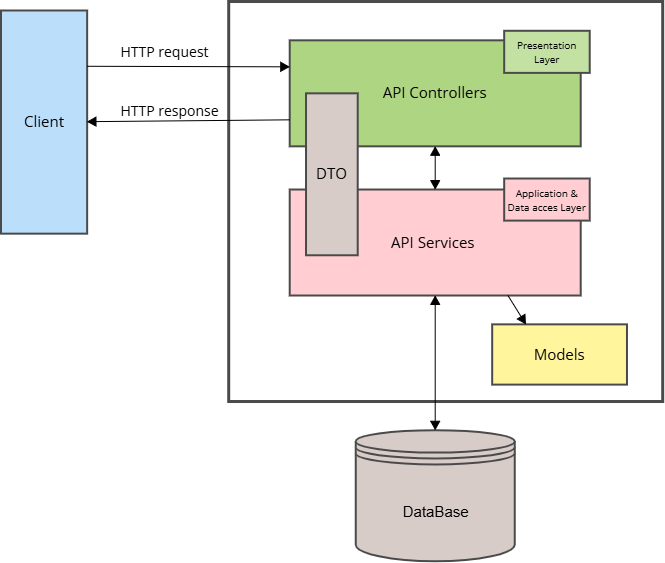
\includegraphics[width=\textwidth]{thesis/files/img/Untitled.png}
    \caption{Architettura \protect\mygls{API}.}
    \label{fig:iarchitettura}
\end{figure}


Questa architettura è stata scelta per questo tipo di struttura per vari motivi, per creare \mygls{API} \mygls{REST} facilmente interrogabili da sistemi \textit{AI}, per garantire una separazione netta delle responsabilità tra i vari livelli aiutando la manutenzione e l'estensione del sistema, proteggere i dati separando i modelli interni con oggetti esposti come i \mygls{DTO}.
Nel contesto del progetto questi sono i livelli principali:
\begin{enumerate}
    \item \textbf{\textit{Presentation layer} - \textit{Controllers}}\\
    I \textit{controller} sono collocati all'interno della cartella \texttt{Controllers} e fungono da punto di contatto tra la logica interna del sistema e l'esterno, nel caso della nostra applicazione il motore di DevLab e il \textit{chatbot}.
    Dentro l'applicazione VisionAI ogni \textit{controller} viene associato a una funzionalità o a un gruppo funzionale, come \texttt{CliForController} che gestisce l'accesso alle anagrafiche clienti/fornitori, o come \texttt{BancheController} che si occupa dell'accesso all'elaborazione dei saldi e dei conti correnti aziendali.
    Ogni \textit{controller} viene incaricato di svolgere diverse operazioni, ricevere richieste \mygls{HTTP} dal motore GPT in formato \textit{GET} o \textit{POST}, valida i parametri in ingresso controllando che siano corretti rispetto alla logica definita, inoltra la richiesta al servizio corrispondente e restituisce una risposta in formato JSON. In questo progetto non esiste una interfaccia utente, il \textit{controller} funge solo da \textit{entry point} per le richieste esterne.
    \item \textbf{\textit{Application} \& \textit{data access layer} - \textit{Services} / \textit{Repository}}\\
    Nel progetto VisionAI la logica applicativa e il \textit{data acces layer} sono stati accorpati in un unica struttura contenuta nella cartella \texttt{Services}, in cui ogni \textit{file} è dedicato in un contesto funzionale differente. Questo approccio ci fa uscire dagli \textit{standard} di un \textit{design pattern} classico, andando a creare una struttura ibrida orientata alla praticità e alla velocità di sviluppo. 
    Ciascun \textit{file} \textit{Repository}, questo il nome dei \textit{file} contenuti nella cartella, ad esempio \texttt{CliForRepository} contiene sia metodi che si occupano della \textit{businnes logic} specifica del dominio (implementazione di parametri e filtri), sia dell'interazione diretta con il \textit{database} utilizzando LINQ o Drapper.
    Come già detto ogni \textit{file} è focalizzato su un area specifica del contesto applicativo, questo consente di avere \textit{repository ad hoc} per ogni gruppo di \mygls{API}.
    \item \textbf{\textit{Data definition} e \textit{transfer} - \textit{Model} / \mygls{DTO}} \\
    Nel progetto VisionAI non viene definito un \textit{layer} apposito per i  \textit{model}, come accade nell'architettura MVC (\textit{Model-View-Controller}) classica. Tuttavia, i \textit{model} svolgono un ruolo essenziale all'interno del nostro sistema, servono a definire come sono strutturati i dati all'interno del \textit{database}, fornendo una rappresentazione diretta delle tabelle.
    Queste classi vengono richiamate all'interno dei \textit{services} per permettere l'interazione con i dati e comprenderne la struttura. A supporto di questa operazione è presente il \textit{file} \texttt{ApplicationDbContext} che definisce il contesto del \textit{database} contenendo le relazioni delle entità interessate, facilitando la navigazione tra le tabelle.
    Oltre a i \textit{model} il progetto utilizza anche \mygls{DTO}, non in maniera globale ma in maniera specifica in alcuni casi, non tutti gli \textit{enpoint} infatti ne fanno uso. Sono stati introdotti per i casi più articolati dove è necessario definire una struttura di risposta standardizzata, controllare l'esposizione evitando la fuoriuscita di dati sensibili e aggregare dati provenienti da tabelle diverse

    \item \textbf{\textit{Database layer}} \\
    Questo \textit{layer} rappresenta lo stato più profondo dell'architettura, in questo strato sono presenti i dati aziendali effettivi. Questi dati sono distribuiti su diversi \textit{database}, tutti in formato SQL Server e preesistenti, i \textit{database} utilizzati sono stati \texttt{VisionEsempio}, \texttt{VisionCommon} e \texttt{VisionAnt}.
    L'accesso alle basi di dati è configurabile nel sistema in modo dinamico tramite l'utilizzo del \textit{file} \texttt{appsetting.json}, il quale contiene le connessioni ai \textit{database} aziendali e i parametri ambientali personalizzabili.
    Durante l'esecuzione l'utente può modificare la connessione ai \textit{database} anche tramite l'utilizzo dell'interfaccia Windows \textit{form} sviluppata.
\end{enumerate}

La progettazione delle \mygls{API} oltre dell'infrastruttura già esistente ha dovuto tenere conto di un altra variabile molto importante, ovvero che queste \mygls{API} non vengono chiamate da un \textit{frontend} programmato per eseguire chiamate standardizzate ma da un \mygls{LLM} che effettua chiamate solamente con il contesto fornitogli da un \textit{prompt}. Questo elemento ha comportato scelte progettuali di grande impatto. Innanzitutto le \mygls{API} sono progettate per essere facilmente interpretabili dal modello mantenendo sempre parametri chiari e assenza totale di ambiguità per i nomi dei campi dati. Inoltre il contesto fornito all'\textit{AI}, in questo caso GPT-4, può essere caricato solamente tramite prompt di testo dalla dimensione limitata, questa caratteristica porta all'impossibilità di costruire \mygls{API} esageratamente complesse o con troppi campi dati per effettuare chiamate molto precise. Diventa quindi di fondamentale importanza la capacità di descrivere il funzionamento delle \mygls{API} in modo riassuntivo e specifico, per fornire il \textit{prompt} corretto e consentire al modello \mygls{LLM} di effettuare una chiamata corretta. Un altro aspetto di estrema importanza progettuale è la robustezza contro \textit{input} imprevedibili, il sistema \textit{backend} quindi deve essere robusto nel controllo degli \textit{input} nelle \mygls{API} POST, effettuando la normalizzazione dei dati, gestendo casi di dati mancanti o inadeguati e gestendo messaggi di errore o comportamenti imprevisti.


\textbf{Progettazione Windows \textit{form}}\\
Nel contesto dell'applicazione VisionAI è stato introdotto un componente accessorio riutilizzabile con l'obiettivo di centralizzare l'accesso all'applicazione in punti specifici all'interno dei prodotti dell'azienda. 
L'obiettivo del \textit{form} è centralizzare l'esecuzione dell'applicativo, infatti rappresenta il punto di ingresso per avviare l'applicazione permettendo di visualizzare e modificare in maniera semplice i dati legati al \textit{database} e alle credenziali d'accesso. Il \textit{form} è stato infatti richiesto per due motivi principali ovvero gestire in modo rapido la connessione al \textit{database} senza dover modificare stringhe a livello codice, e supportare configurazioni lanciando l'\textit{app} in modo diretto dal gestionale e permettendo all'utente di salvare i propri dati di accesso e riutilizzarli all'interno di sessioni successive.
L'utilizzo di Windows \textit{form} è stata richiesta in modo diretto dall'azienda, mantenendo un interfaccia semplice focalizzata sulla  connessione all'\textit{app} vera e propria.
Per garantire la connessione al \textit{database} viene modificato in modo diretto il \textit{file} \texttt{appsetting.json}, che contiene tutte le stringhe di connessione.
Per quanto riguarda invece la gestione delle credenziali e delle sessioni di accesso il discorso è più lungo.
Questa sezione ha l'obiettivo di mantenere la connessione alla \textit{chat} anche in caso la connessione venga interrotta a causa delle sessioni a tempo. Risulta scomodo l'inserimento delle credenziali in maniera manuale ogni trenta minuti.
Per risolvere questo problema è stato aggiunto al \textit{form} una sezione che consente l'inserimento delle credenziali iniziali, esegue la chiamata di \textit{login} e ottiene in  risposta due \textit{token} uno di accesso e uno di \textit{refresh}. Questi due \textit{token} vengono salvati in \textit{file} locali in particolare: 
\begin{itemize}
    \item \texttt{log.json}: salva il \textit{token} di accesso alla sessione che sta per essere avviata.
    \item \texttt{ses.json}: salva il \textit{token} di \textit{refresh}, utilizzato per aggiornare la sessione corrente senza il reinserimento dei dati.
    \item \texttt{data.json}: registra l'orario della generazione dei \textit{token}.
\end{itemize}
Ogni sessione ha la durata \textit{standard} di trenta minuti e per garantire quindi continuità nell'uso della \textit{chat}, viene letto il valore temporale di \texttt{data.json}, se sono trascorsi più di trenta minuti il sistema esegue automaticamente una chiamata di \textit{refresh} e sovrascrive i \textit{token} precedenti con quelli nuovi ricevuti come risposta.

\subsection{Difficoltà incontrate durante la codifica}
Lo sviluppo delle \mygls{API} per VisionAI ha richiesto un attività di codifica approfondita, caratterizzata anche dai vincoli strutturali imposti dalla base dati esistente e dall'architettura predefinita. 
Una delle complessità principali è stata la gestione dell'accesso a dati distribuiti su più tabelle relazionate. Praticamente tutte le \mygls{API} sviluppate nel periodo infatti chiedevano la risposta a domande complesse e per garantire ciò era necessario accedere a dati provenienti da entità diverse. Per affrontare queste difficoltà è stato adottato Entity Framework Core, un \mygls{ORM} che contente di eseguire \textit{query} SQL in maniera astratta tramite LINQ-to-Entities, questo approccio ha permesso di gestire le relazioni tra tabelle attraverso \textit{join} espliciti all'interno del codice ma senza usare codice SQL, applicare filtri dinamici per permettere l'utilizzo di parametri all'interno della chiamata, recuperare e proiettare i dati in strutture che poi vengono trasformate in \mygls{DTO}. È possibile visualizzare il funzionamento ad alto livello di un sistema \mygls{ORM} nella figura \ref{fig:ORM}.
Particolare attenzione è stata dedicata anche alla validazione dei dati in \textit{input} per quanto riguarda le \mygls{API} \textit{POST}, effettuando controlli sui campi obbligatori, normalizzando i dati prima dell'inserimento nel \textit{database} e aggiornando lo \textit{script} di assegnazione automatica del campo \texttt{CodCliFor} applicando l'algoritmo di assegnazione aziendale.

\begin{figure}[H]
    \centering
    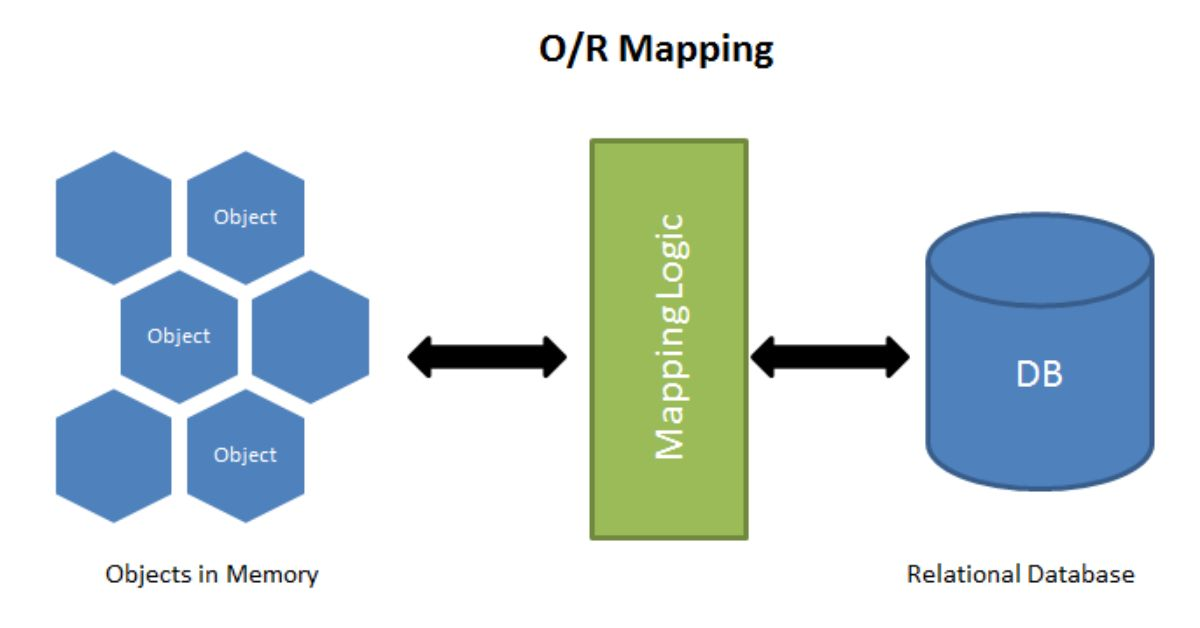
\includegraphics[width=.7\columnwidth]{thesis/files/img/ORM.jpg}
    \caption[Diagramma di funzionamento di un ORM.]{
        Diagramma di funzionamento di un ORM.\\
\textit{Fonte:\url{https://www.youstable.com/it/blog/cos'è-ORM-nella-programmazione/}}
    }
    \label{fig:ORM}
\end{figure}




\subsection{Verifica e presentazione dei risultati ottenuti}
La verifica ha rappresentato un'attività molto importante del processo di sviluppo, al fine di garantire la correttezza e coerenza delle funzionalità implementate.
Sebbene, per motivi di tempo, non siano stati introdotti \textit{test} automatici strutturati, ho condotto un'attenta validazione manuale di tutte le \mygls{API} sviluppate, sia negli ambienti locali sia nell'integrazione con il \textit{chatbot}.\\
\textbf{\textit{Test} funzionali delle \mygls{API}} \\ 
Ogni \mygls{endpoint} è stato \textit{testato} singolarmente mediante strumenti di ispezione delle \mygls{API} tra cui Swagger, utilizzato durante lo sviluppo per l'esposizione degli \textit{enpoint}, il controllo dei parametri, la correttezza delle risposte \mygls{HTTP} e la visualizzazione della documentazione interattiva delle \mygls{API}. Altro strumento utilizzato è stato Postman, impiegato per simulare chiamate reali dinamiche tramite OData, per visualizzare le risposte in formato JSON.
Per ogni \mygls{API} sviluppata è stato verificato: 
\begin{itemize}
    \item il corretto \textit{routing},
    \item la validità dei parametri e la logica a loro collegata,
    \item la coerenza delle risposte con i dati effettivamente presenti nel \textit{database},
    \item la corretta gestione degli errori,
    \item coerenza dei dati rispetto la logica richiesta.
\end{itemize}
Oltre all'integrazione di \textit{test} locali tramite gli strumenti citati, sono stati svolti \textit{test} sull'integrazione effettiva delle \mygls{API} con l'assistente utilizzando Ngrok per esporre il \textit{backend} locale rendendolo accessibile al motore esterno di DevLab.
Al termine delle attività sono state sviluppate con successo una serie di nuove \mygls{API} che integrano funzionalità e permettono all'assistente virtuale di rispondere in modo corretto a domande collegate a nuovi contesi.
Nella tabella \ref{tab:api-sviluppate} presento tutte le \mygls{API} sviluppate e sistemate.

\begin{table}[H]
\centering
\begin{tabular}{|p{5cm}|p{3cm}|p{4cm}|}
\hline
\textbf{Nome API} & \textbf{Metodo} & \textbf{Tipologia} \\
\hline
Dipendenti (Anagrafiche Dipendenti) & \textit{GET / POST} & Nuova \\
\hline
Banche (Saldi Conti Correnti) & \textit{GET} & Nuova \\
\hline
Ordini Evasi / Non Evasi & \textit{GET} & Nuova \\
\hline
Manutenzioni da Eseguire & \textit{GET} & Nuova \\
\hline
Manutenzioni per Destinazione & \textit{GET} & Nuova \\
\hline
SqlTraducer & \textit{GET} & Aggiornata \\
\hline
CliFor (Clienti/Fornitori) & \textit{GET / POST} & Aggiornata \\
\hline
Contatti (Anagrafiche Contatti) & \textit{GET / POST} & Aggiornata \\
\hline
Attivit\`a & \textit{GET / POST} & Aggiornata \\
\hline
\end{tabular}
\caption{API sviluppate e sistemate durante il periodo di stage.}
\label{tab:api-sviluppate}
\end{table}


\textbf{Windows \textit{from}}\\
Anche per il Windows \textit{form} non sono stati effettuati dei \textit{test} automatici ma abbiamo controllato le funzionalità verificando l'avvio dell'applicazione, la corretta modifica delle stringhe di connessione al \textit{database}, il salvataggio di una nuova connessione ad un nuovo \textit{database} e funzionalità collegate alla semplice interfaccia sviluppata che è possibile visualizzare nell'immagine \ref{fig:interfaccia-form}.

\begin{figure}[H]
    \centering
    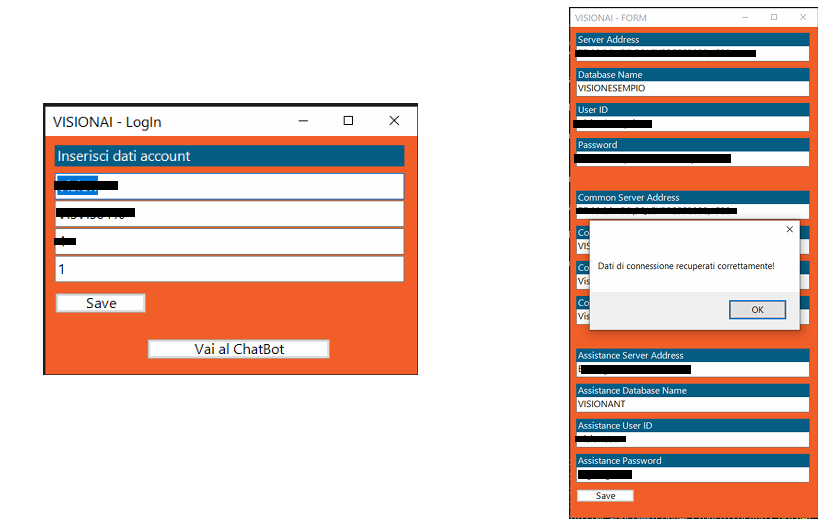
\includegraphics[width=\textwidth]{thesis/files/img/FORM-FINALE.PNG}
    \caption{Interfaccia finale \textit{form}.}
    \label{fig:interfaccia-form}
\end{figure}



\section{Sistema di assegnazione automatica per VisionAssistance}
Lo sviluppo del modulo di assegnazione automatica ha rappresentato una delle sfide più articolate e stimolanti dell'esperienza di \textit{stage}. L'obiettivo principale era quello di progettare un sistema in grado di rendere automatica l'assegnazione degli interventi ottimizzando una serie di variabili temporari, logistiche e contrattuali.
Data la complessità del dominio e l'alto numero di vincoli da rispettare si è deciso di affrontare il problema mediante la realizzazione di un \mygls{PoC},prodotto incompleto per dimostrare la fattibilità, tipo un prototipo, producendo un prodotto funzionante ma limitato.

\subsection{Analisi dei requisiti}
L'attività di definizione e raccolta dei requisiti si è basata su una stretta collaborazione con il \textit{tutor} aziendale e con il \textit{team} interno di VisioneImpresa. I requisiti sono stati definiti partendo da una serie di specifiche fornite in forma di documenti e integrate con vari incontri informali e sessioni di chiarimento con personale specializzato nel contesto di VisionAssistance. 
Alla base dei requisiti si pone l'obiettivo creare un sistema di l'assegnazione automatica dei tecnici agli interventi da svolgere, effettuando una pianificazione compatibile con diverse variabili come le disponibilità temporali dei tecnici e dei clienti, i vincoli contrattuali, le distanze fisiche, i tempi di spostamento e la priorità .

Nella tabella \ref{tab:req-agent} sono contenuti tutti i requisiti individuati, il codice viene definito nel seguente modo: 
\begin{center}
\textbf{R[\textit{O/D/F}]-NN}
\end{center}

dove:
\begin{itemize}
  \item \textbf{R} indica che si tratta di un requisito;
  \item \textbf{O/D/F} specifica il grado di priorità:
    \begin{itemize}
      \item \textbf{O}: Obbligatorio – deve essere implementato;
      \item \textbf{D}: Desiderabile – migliora il sistema ma non è essenziale;
      \item \textbf{F}: Facoltativo – implementabile solo in caso di tempo o risorse aggiuntive.
    \end{itemize}
  \item \textbf{NN} è un numero progressivo per identificare univocamente ogni requisito.
\end{itemize}

\begin{longtable}{|c|p{13.5cm}|}
\hline
\textbf{Codice} & \textbf{Descrizione} \\
\hline
RO-01 & Rispettare orari di apertura e giorni lavorativi specificati dal cliente tramite la tabella \texttt{P\_Orari}. \\
\hline
RO-02 & Considerare gli orari lavorativi settimanali dei tecnici contenuti nella tabella \texttt{CalendSett}. \\
\hline
RO-03 & Rispettare festività e orari speciali contenuti nella tabella \texttt{CalendDay}. \\
\hline
RF-04 & Utilizzare \textit{Google Places \mygls{API}} per verificare apertura delle attività. \\
\hline
RO-05 & Aggiungere tempo amministrativo fisso o in percentuale configurato per ogni intervento. \\
\hline
RO-06 & Pianificare interventi solo in presenza di sovrapposizione oraria tra cliente e tecnico. \\
\hline
RO-07 & Considerare partenza del tecnico dalla sede aziendale di appartenenza. \\
\hline
RO-08 & Mantenere orario se la data prevista è futura, ricalcolare se è già trascorsa. \\
\hline
RO-09 & Rispettare l'assegnazione del tecnico da contratto se presente. \\
\hline
RD-10 & Se il tecnico del contratto differisce da quello del buono, sostituirlo con quello corretto. \\
\hline
RD-11 & Consentire la sostituzione del tecnico solo se non vincolato da contratto. \\
\hline
RO-13 & Supportare assegnazioni spezzate per interventi di lunga durata. \\
\hline
RF-14 & Prevedere \textit{fallback} in caso di assenza di tecnici disponibili. \\
\hline
RD-15 & Generare \textit{output} in formato JSON.  \\
\hline
\caption{Tabella dei requisiti individuati per il modulo di assegnazione interventi.}
\label{tab:req-agent}
\end{longtable}

\subsection{progettazione}
Come anticipato nella sezione \ref{sec:pianificazione-attività} per motivi legati ai tempi del progetto, abbiamo deciso di dividere il lavoro, io mi sono concentrato principalmente sulla progettazione e implementazione della \textit{pipeline} dei dati.
Questa parte del progetto costituisce la base di informazioni su cui opera l'algoritmo di assegnazione automatica sviluppato in parallelo dal mio collega.
La progettazione ha seguito principi di modularità e riusabilità e disaccoppiamento delle responsabilità, come è visibile anche solo a livello di struttura della \textit{repository} nella figura \ref{fig:atruttura-pipeline} fissando come obiettivi principali:
\begin{itemize}
    \item Modularità del sistema, ogni componente svolge un compito preciso e può essere modificato indipendentemente.
    \item Automazione del flusso dei dati, la \textit{pipeline} è progettata per essere avviata con un unico comando.
    \item Standardizzazione, l'\textit{output} di questo modulo è standardizzato per essere compatibile con il sistema di assegnazione automatica.
    \item Estensibilità, la struttura modulare permette l'aggiunta di nuovi componenti in maniera semplice senza modificare la logica esistente.
\end{itemize}

\begin{figure}[H]
    \centering
    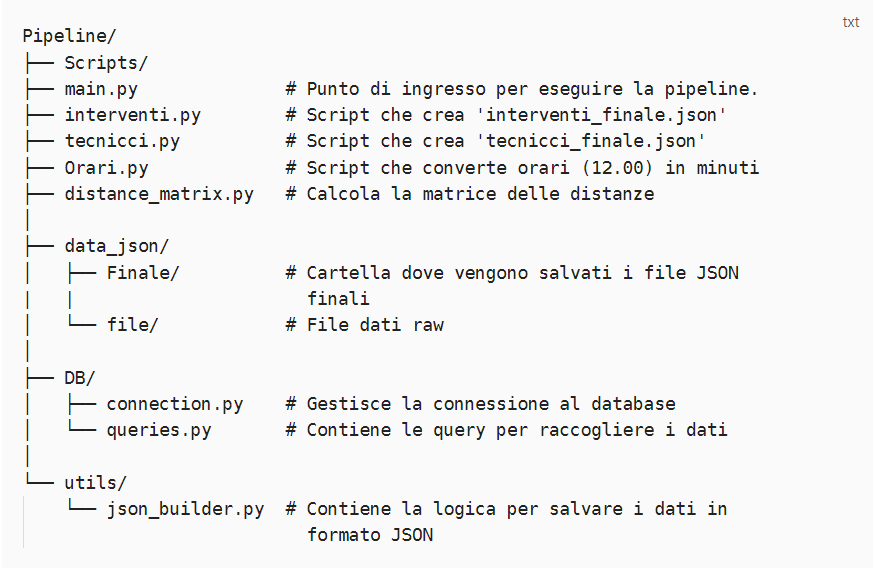
\includegraphics[width=\textwidth]{thesis/files/img/Cattura.PNG}
    \caption{Struttura delle \textit{repository} della \textit{pipeline}.}
    \label{fig:atruttura-pipeline}
\end{figure}

Dal punto di vista architetturale la \textit{pipeline} è organizzata in moduli indipendenti come si può visualizzare nella figura \ref{fig:giagram-pip}, sviluppati in Python e raggruppati in diverse cartelle come \texttt{Scripts}, \texttt{DB} e \texttt{data\_json}, ogni modulo svolge un passaggio chiave:
\begin{itemize}
    \item \texttt{Connection}: stabilisce la connessione con il \textit{database} SQL Server utilizzando SQLAlchemy e Pyodb, riunendo tutta la gestione delle variabili di accesso.
    \item \texttt{Queries}: contiene tutte le \textit{query} SQL utilizzate per estrarre tutti i dati necessari al fine di creare una base dati robusta per l'algoritmo di assegnazione.
    \item \texttt{Interventi}: modulo che si occupa di normalizzare tutti i dati relativi agli interventi da svolgere, gestendo vincoli, priorità, orari dei clienti e posizioni, andando a produrre il \textit{file} \texttt{interventi\_finale.json}.
    \item \texttt{Tecnici}: modulo che in maniera simile a quello degli interventi va a organizzare e normalizzare tutti i dati relativi ai tecnici andando a creare il \textit{file} \texttt{tecnici\_finale.json}.
    \item \texttt{Orari}: modulo che si occupa di convertire gli orari in minuti, per semplificare la manipolazione temporale nella sezione di \textit{scheduling}.
    \item \texttt{Distance\_matrix}: Modulo che si occupa di calcolare le distanze (in minuti) tra sedi e interventi utilizzando le \mygls{API} \textit{Google Maps Distance Matrix}, producendo il \textit{file} \texttt{distance\_matrix.json}.
\end{itemize}

\begin{figure}[H]
    \centering
    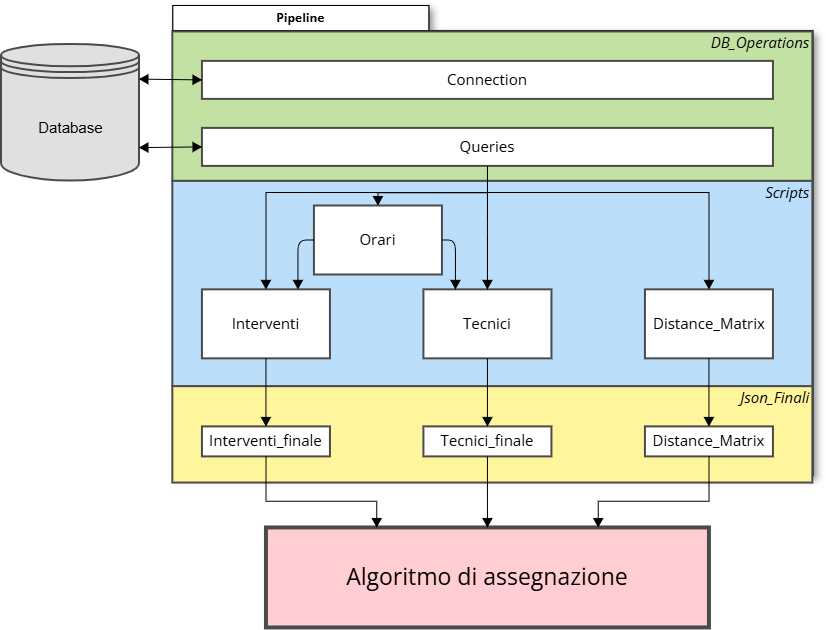
\includegraphics[width=\textwidth]{thesis/files/img/pip.png}
    \caption{Struttura architetturale della \textit{pipeline} dei dati.}
    \label{fig:giagram-pip}
\end{figure}

Nella tabella \ref{tab:scelte-chiave-agent} vengono presentate le scelte progettuali ritenute chiave.

\begin{table}[H]
\centering
\begin{tabular}{|p{4cm}|p{10cm}|}
\hline
\textbf{Decisione} & \textbf{Motivazione} \\
\hline
Linguaggio \texttt{Python} & Facilita l'integrazione, lo sviluppo rapido e l'uso di librerie avanzate per l'elaborazione dati. \\
\hline
SQLAlchemy + ODBC & Permette \textit{query} flessibili e sicure su SQL Server con gestione centralizzata delle connessioni. \\
\hline
\textit{Script} modulari & Ogni parte della \textit{pipeline} è isolata e facilmente modificabile/\textit{testabile}. \\
\hline
Gestione orari in minuti & I dati temporali sono convertiti in formato numerico per ottimizzare la gestione dei vincoli nell'algoritmo. \\
\hline
\textit{Google Distance Matrix \mygls{API}} & Calcolo realistico dei tempi di viaggio. \\
\hline
\end{tabular}
\caption{Scelte progettuali chiave adottate nella realizzazione della \textit{pipeline}.}
\label{tab:scelte-chiave-agent}

\end{table}

\subsection{Verifica e risalutati ottenuti}
La verifica per il modulo di \textit{pipeline} dei dati ha rappresentato  un'attività fondamentale per garantire la correttezza delle informazioni generate, che venendo poste alla base dell'algoritmo di decisione dei tecnici, è di estrema importanza quindi la verifica della corretta presentazione. 
Per questa sezione essendo anche un \mygls{PoC} non abbiamo introdotto sistemi di \textit{testing} automatici o semiautomatici incentrando la fase di verifica sulla validazione funzionale dei singoli script e assicurandosi che l'\textit{output} fosse coerente con i dati nel \textit{database} e integrabile con il modulo di \textit{scheduling}.

Sono stati fatti quindi \textit{test} manuali sistematici, che si concentrano sulla coerenza e la qualità dei dati prodotti. 
\begin{itemize}
    \item Controllo diretto delle \textit{query} SQL: ogni \textit{query} eseguita nel processo di estrazione dei dati è stata confrontata con i dati reali presenti nel \textit{database}, per verificarne la corrispondenza e la coerenza.
    \item Verifica dei dati aggregati: i \textit{file} JSON generati sono stati analizzati manualmente per accertare che ogni informazione fosse coerente rispetto all'origine nel \textit{database} e non ci fossero dati nulli non giustificati.
    \item Validazione del processo di trasformazione dei dati: sono state verificate le strutture dati finali per assicurare che riflettessero in maniera corretta quanto previsto in fase di progettazione
    \item Matrice delle distanze: Una attenzione maggiore è stata dedicata alla verifica della matrice dei tempi di percorrenza tra le sedi e i luoghi di intervento. Sono stati effettuati diversi \textit{test} per verificare la correttezza degli indirizzi presi in considerazione per il calcolo delle distanze, avvenuto un controllo a campione della correttezza dei tempi di viaggio restituiti, assicurare la funzionalità del sistema \textit{testando} la divisione in chiamate per rispettare i limiti imposti da Google e la gestione delle risposte \texttt{null}.
\end{itemize}


La \textit{pipeline} dei dati sviluppata è stata integrata nel \mygls{PoC}, questa unione ha confermato la corretta realizzazione di essa, in quanto tutti i \textit{file} JSON prodotti sono risultati compatibili con l'algoritmo di pianificazione, l'elaborazione dei dati ha portato a risultati concreti in rispetto dei vincoli imposti e l'\textit{output} dell'algoritmo ha evidenziato una risposta funzionale coerente pur essendo in uno scenario di prova.
L'intero lavoro si è tradotto quindi nella realizzazione di un prototipo funzionante concreto, che dimostra la fattibilità e la possibile integrazione futura nei prodotti aziendali. Per quanto riguarda i requisiti inizialmente individuati, i requisiti obbligatori sono stati tutti integrati assicurando che il sistema di assegnazione dei tecnici rispettasse i vincoli imposti mentre i requisiti desiderabili e facoltativi non sono stati integrati nel sistema.
\newpage
    \chapter{Valutazione retrospettiva}
\label{chap:Valutazione-Retrospettiva}

\section{Valutazione degli obiettivi}
\subsection{Obiettivi  aziendali}
Gli obiettivi aziendali rivolti al progetto di \textit{stage} erano diversi e distribuiti sui due moduli differenti che ne facevano parte. Come indicato all'interno della tabella \ref{tab:obiettivi-aziendali} e \ref{tab:obiettivi-aziendali-interventi}, gli obiettivi per questi progetti erano divisi in obbligatori, desiderabili e facoltativi.

Nel caso del modulo legato all'estensione del raggio di competenza della \textit{chatbot} aziendale chiamata VisionAI, ho raggiunto pienamente i due obiettivi obbligatori:
\begin{itemize}
	\item O001: sviluppo di interfacce con DevExpress - l'interfaccia Windows \textit{form} è stata implementata con successo, contenendo tutte le funzionalità richieste come connessione diretta alla \textit{chat} salvando i dati e le sessioni e modificare e aggiungere connessioni ai \textit{database} 
	\item O002: sviluppo \mygls{API} \mygls{REST} in C\# - ho contribuito attivamente allo sviluppo delle nuove \mygls{API} ma anche alla correzione di quelle esistenti, al fine di estendere la funzionalità dell'assistente VisionAI. Tutte le \mygls{API} le ho  sviluppate seguendo l'architettura definita dall'azienda utilizzando ASP.NET Core. 
\end{itemize}
Ho raggiunto anche l'obiettivo D01 che comprendeva la documentazione e il piano dei \textit{test}, seppur in parte, vista l'assenza di una \textit{suite} di \textit{test} automatici, compensato però da una rigida verifica manuale delle funzionalità e una documentazione dettagliata.
Per quanto riguarda il modulo legato al contesto di VisionAssistance, l'obiettivo indicato dall'azienda era facoltativo, F01 ovvero la creazione di un \textit{agent} per la pianificazione automatica degli interventi, questo obiettivo è stato raggiunto sotto forma di \mygls{PoC} che ha dimostrato la fattibilità del progetto, rispettando i vincoli imposti e dando risposte coerenti.

In generale ho realizzato tutti gli obiettivi aziendali, ottenendo anche un buono stato di soddisfacimento da parte del referente aziendale al momento della presentazione del lavoro svolto.

\subsection{Obiettivi  personali}
Prima che iniziasse lo \textit{stage}, mi ero posto alcuni obiettivi personali con l'intenzione di sfruttare l'esperienza per apprendere molto sia dal un punto di vista formativo che umano.
Gli obiettivi che mi sono posti non erano riguardanti solo l'acquisizione di competenze tecniche, ma anche il modo in cui volevo affrontare il lavoro in un contesto aziendale.

Uno degli aspetti riguardava la volontà di apprendere nuove tecnologie, in particolare legate all'ambiente di .NET e allo sviluppo in linguaggio C\#. Provenendo da un ambiente accademico incentrato molto sulla teoria mi interessava  ampliare il mio \textit{stack} tecnologico con soluzioni legate prettamente al mondo del lavoro. Lavorare su un progetto reale utilizzando queste tecnologie mi ha permesso di crescere molto.
Un altro obiettivo importante per me era quello di sviluppare un metodo di lavoro, imparando a pianificare le attività rispettare le scadenze e avere un flusso di lavoro continuo e positivo. Volevo seguire una struttura ben definita organizzandomi le cose da fare e arrivando a terminare il lavoro senza ritardi e difficoltà e il contesto aziendale si è rivelato molto utile per raggiungere questo obiettivo.
Avevo inoltre la volontà di rafforzare le mie capacità relazionali, sia all'interno del \textit{team} di sviluppo sia nel confronto con altri membri dell'azienda. La possibilità di collaborare al progetto è stata molto importante, permettendomi di lavorare sempre insieme a qualcuno migliorando molto le mie capacità comunicative e rendendo il progetto più interessante.
Infine uno degli aspetti che ritenevo più importanti era quello di mettermi alla prova in un ambiente lavorativo, allontanandomi dalla zona di \textit{comfort} dell'università. Ho cercato di affrontare con positività nuove situazioni e a valorizzare questa esperienza come possibilità di crescita.
Per concludere posso confermare che gli obiettivi personali sono stati raggiunti in modo pieno, ho trovato questa esperienza molto formativa sotto sia il punto di vista tecnico che umano.


\section{Conoscenze e competenze acquisite}
Durante il periodo di \textit{stage} ho avuto la possibilità di imparare moltissimo accrescendo il mio bagaglio tecnico e di competenze trasversali, l'esperienza è stata anche più ricca di quanto mi aspettassi poiché mi ha permesso di lavorare su progetti complessi e concreti e con tecnologie utilizzate nel mondo del lavoro.
Uno degli aspetti più importanti se parliamo di competenze acquisite è sicuramente l'ambiente .NET e il linguaggio C\#, che ho utilizzato in maniera quotidiana per lo sviluppo del \textit{backend} di VisionAI. Pur avendo qualche nozione di base durante lo \textit{stage} ho appreso l'organizzazione di un vero progetto aziendale con un architettura a strati e l'importanza di alcuni concetti base per la scrittura di un buon codice. In particolare ho appreso familiarità con lo sviluppo di \mygls{API} tramite ASP.NET Core, la progettazione di un sistema \textit{controller, repository e service} e l'utilizzo di tecnologie e \textit{framework} correlate all'ambiente .NET.
Ho imparato molto anche dal punto di vista del lavoro con \textit{database}, lo \textit{stage} ha rappresentato proprio un salto di livello. Pur partendo con una base di nozioni solida sia per quanto riguarda SQL sia per quanto riguarda il \textit{database}, confrontarmi con una base di dati complessa e un sistema di grandi dimensioni basato sulle relazioni tra tabelle mi ha portato a sviluppare competenze più avanzate. Sicuramente ho imparato a scrivere \textit{query} complesse, lavorare con un \textit{database} di grandi dimensioni comprendendone la struttura e utilizzare SQL Server Management Studio come strumento quotidiano.
Oltre a questi ho potuto utilizzare molti altri strumenti come Google Or-Tools e apprndere nozioni sulla programmazione vincolata, utilizzare \mygls{ORM} come Entity framework e SQLAlchemy conoscendo molte nuove tecnologie e soluzioni.
Oltre alle competenze tecniche lo \textit{stage} mi ha permesso di crescere anche con abilità trasversali fondamentali per il mondo del lavoro, come il lavorare in \textit{team} in maniera continuativa, confrontandomi ogni giorno con un altra persona e condividendo idee e problemi. Migliorare sotto il punto di vista comunicativo e di organizzazione del lavoro, relazionarmi con un ambiente lavorativo e tutte le dinamiche interne. Tutte queste competenze e conoscenze che ho appreso in questo periodo le reputo molto preziose.

\section{Considerazioni finali sul percorso universitario}
Il percorso universitario che ho affrontato è stato sicuramente impegnativo e con molti ostacoli, allo stesso tempo però molto stimolante e costruttivo. Questi anni all'interno dell'ambiente universitario sono stati molto formativi non solo dal punto di vista di apprendimento ma anche dal punto di vista metodologico e umano, e tornassi indietro sceglierei ancora questo percorso consapevole del valore che mi ha restituito.
Durante questo periodo, lavorando all'interno di un'azienda e partecipando in maniera attiva a progetti veri mi sono reso conto che l'università ti prepara al mondo del lavoro, anche se in un modo meno diretto di quello che si può pensare. Non ti insegna ad usare ogni strumento o a conoscere ogni linguaggio, sarebbe impossibile, soprattutto nel mondo dell'informatica che è in continua evoluzione.
Quello che invece ti offre è una base molto solida di conoscenze teoriche e un metodo di ragionamento. Ti insegna come imparare, come risolvere problemi e a risolverli da solo.
Con questa esperienza ho capito in modo significativo di quanto le basi siano essenziali, perché senza fondamenta non si costruisce niente di solido.
In informatica imparare come affrontare un problema, anche senza conoscere a priori la tecnologia, è più importante che conoscere la tecnologia stessa e questo è alla base di questa università.


\newpage



    \cleardoublepage
\appendix
\pagenumbering{roman} % Imposta numeri romani PRIMA di settare il numero
\setcounter{page}{1}  % Solo se vuoi che il Glossario inizi da i (opzionale)
\phantomsection
\addcontentsline{toc}{chapter}{Glossario}
\chapter*{Glossario}


\begin{description}
  \item[\hypertarget{gls:API}{API}] (Application Program Interface) In un programma informatico per \textit{API} si intende un insieme di definizioni o protocolli che permettono a componenti \textit{software} di comunicare con altri componenti \textit{software} e scambiarsi dati. Le \textit{API} permettono la condivisione solo dei dati necessari mantenendo nascosti i dettagli interni del sistema. 

  \item[\hypertarget{gls:ERP}{ERP}] Un \textit{enterprise resource planning} è un tipo di \textit{software} di gestione che integra tutti i processi aziendali come vendite, acquisti, gestione magazzino, finanza e contabilità. I sistemi \textit{ERP} centralizzano i dati provenienti da un insieme di processo di \textit{business} rendendoli disponibili a tutti. Oggi i sistemi \textit{ERP} risultano fondamentali per la gestione delle aziende.
  
  \item[\hypertarget{gls:PBX}{PBX}] Un \textit{private branch exchange} nelle telecomunicazioni è una rete telefonica privata che viene usata all'interno di un azienda o organizzazione. Questa infrastruttura permetta la comunicazione interna ed esterna. Un \textit{PBX} consente di avere più telefoni rispetto alle linee telefoniche fisiche e consente chiamate gratuite tra gli utenti. 
  
  \item[\hypertarget{gls:IDE}{IDE}] Con \textit{integrated development environment} o ambiente di sviluppo integrato si intende un \textit{software} progettato per la realizzazione di applicazioni che riunisce diversi strumenti di sviluppo in un unica interfaccia grafica. Costituito da un \textit{editor} di codice sorgente, un automazione della \textit{build} locale e un \textit{debugger}. 
  
  \item[\hypertarget{gls:REST}{REST}] \textit{Representational state transfer} si tratta di un architettura\textit{software} che impone condizioni sul funzionamento di un \textit{API}.  Si utilizza l'architettura basata su \textit{REST} per supportare comunicazioni affidabili e con alte prestazioni su larga scala. Gli sviluppatori di \textit{API} possono progettarle utilizzando diverse architetture e quelle che seguono le architetture \textit{REST} sono chiamate \textit{RESTful}.
  
  \item[\hypertarget{gls:ORM}{ORM}] \textit{Object-relational mapping} nell'informatica è un \textit{pattern} di programmazione che crea un ponte virtuale tra tra il paradigma orientato agli oggetti e il modello relazionale dei \textit{database}, permettendo agli sviluppatori di manipolare dati ed effettuare chiamate utilizzando gli oggetti nel linguaggio di programmazione corrente senza inserire codice in SQL. 
  
  \item[\hypertarget{gls:DTO}{DTO}] \textit{data transfer object} è un oggetto che definisce le modalità di invio dati in rete o tra sottoinsiemi di un applicazione software, rendendo possibile mappare i dati che si voglio trasferire nascondendo quelli non opportuni o sensibili. 
  
  \item[\hypertarget{gls:HTTP}{HTTP}] \textit{Hypertext Transfer Protocol} è un protocollo di comunicazione alla base della trasmissione di dati sul \textit{web}, e definisce i comandi e i servizi utilizzati per il trasferimento dei dati in rete.
   
  
  \item[\hypertarget{gls:LLM}{LLM}] \textit{large language model}, in italiano modello linguistico di grandi dimensioni,è una tecnologia molto avanza nell'ambito \textit{AI}, incentrata sulla comprensione, l'analisi e la generazione del testo in ambito generale.
   
  
  \item[\hypertarget{gls:PoC}{PoC}] \textit{proof of concept} ha lo scopo di determinare la fattibilità dell'idea e verificare che l'idea funzionerà come previsto. Può essere visto come una fase di \textit{test} iniziale dell'idea e come un prototipo.

  
  \item[\hypertarget{gls:legacy}{Legacy}]  Un sistema \textit{legacy} in informatica è un sistema utilizzati per un periodo prolungato che generalmente presenta una tecnologia obsoleta, prestazioni inefficienti, vulnerabilità di sicurezza, costi di manutenzione elevati, scalabilità limitata e scarsa attendibilità.
  
  
  \item[\hypertarget{gls:endpoint}{Endpoint}] un \textit{endpoint} è un luogo digitale in cui un \textit{API} riceve chiamate, note come richieste, per le risorse sul suo \textit{server}. Gli \textit{endpoint} sono complementari alle \textit{API} e si presentano molto spesso sotto forma di \textit{URL}.
  
  
  \item[\hypertarget{gls:Clean architecture}{Clean architecture}] Il termine \textit{Clean architecture} deriva dall'omonimo libro di Robert C. Martin e possiamo pensarla come un insieme di linee guida per progettare l'architettura di un \textit{software}. I suoi principi si possono riassumere in indipendenza dal \textit{framework}, indipendenza dall'\textit{UI}, indipendenza dal \textit{database} e \textit{testabile}.
  
\end{description}

\cleardoublepage
\pagenumbering{roman}

    
    %\pagenumbering{roman}
    \backmatter

    %\printglossary[type=\acronymtype, title=Acronimi e abbreviazioni, toctitle=Acronimi e abbreviazioni]
    %\printglossary[title=Glossario, toctitle=Glossario]
    \setcounter{page}{4}
    \chapter{Sitografia}
\label{cap:webliography}
\nocite{*}

% Websites bibliography
\printbibliography[heading=subbibliography, title={\null}, type=online]

\end{document}